\titleformat{\chapter}[display]
{\normalfont\Large\bfseries}{Appendix~\Alph{chapter}}{11pt}{\Large}
\appendix
\renewcommand{\thechapter}{\Alph{chapter}}
\chapter{Vector Calculus}
\section{指标运算}
指标运算其实就是在涉及到向量, 张量求和表示时, 频繁的使用$\Sigma$会降低文章的可读性, 索性人为的\uwave{规定}去掉求和符号。
\begin{proposition}{爱因斯坦求和约定}
    只要是某一项中出现的两个相同的指标\footnote{$\bigstar$不可能在某一项中出现三个相同的指标。}, 那么就理解为对这个指标求和也就是说
    \begin{center}
        \begin{math}
            \displaystyle
            c_i = \sum_{j=1}^{3}a_{ij}b_{j} \Longleftrightarrow c_i=a_{ij}b_{j} \text{\quad} (i=1,2,3)
        \end{math}
    \end{center}
    我们称$j$为\uwave{哑指标},$i$为\uwave{自由指标}, 总的来说, 这就是一种方便使用的约定记号, 而且有时候去掉求和符号后能够是我们更加清晰地进行计算。
\end{proposition}
指标运算这个东西实际上非常微妙, 一方面它能帮助你大幅度的简化运算, 另一方面它的一些操作总是让人头晕。关于哑指标和自由指标, 你需要记住的就是哑指标只是
表示求和, 所以你可以更换字母或者对换字母, 例如:$a_ib_i=a_jb_j$, $a_{ij}b_{ji}=a_{ji}b_{ij}(i\leftrightarrow j)$, 而自由指标更像是在表示某个向量
的某一个分量, 你需要对等式两边同时去替换。
\begin{define}{符号定义}
    1.克罗内克符号(Kronecker delta)\qquad\qquad
    
    \begin{math}
        \centering
        \delta_{ij}=\begin{cases}
            0,& i \neq j\\
            1,& i=j
        \end{cases}
    \end{math}\\
    2.列维-奇维塔符号\footnote{$\tau$表示逆序数}(Levi-Civita symbol)\\
    \begin{center}
    \begin{math}
        \epsilon_{ijk}=\begin{cases}
            1,&\tau(ijk)\text{ is even}\\
            -1,&\tau(ijk)\text{ is odd}\\
            0,&\text{any of $i,j,k$ is equal}
        \end{cases}
    \end{math} 
    \end{center}
\end{define}    
克罗内克符号常常被用来\uwave{替换指标}, 下面的关系在简化运算时非常有用。
\begin{lequation}
    \boxed{
        \delta_{ij}a_j=a_i \qquad \qquad \delta_{ij}a_{jk}=a_{ik}
    }
\end{lequation}

也就是说一旦碰到相同的指标$\delta$会将那一项的这个指标替换为$\delta$的另一个指标, 比如上面的公式$\delta$作用为$j\leftrightarrow i$。

$\epsilon$和$delta$之间有一个十分有用的关系式:
\begin{lequation}
    \boxed{
        \epsilon_{ijk}\epsilon_{klm}=\delta_{il}\delta_{jm}-\delta_{im}\delta_{jl}
    }
\end{lequation}
\begin{thinknote}
    \textbf{几个使用求和约定表示的例子:}\\
    \begin{math}
        \displaystyle
        \bm{a}\cdot\bm{b}=a_ib_i \qquad\qquad [\bm{a}\times\bm{b}]_i=\epsilon_{ijk}a_jb_k\\
        \left(\bm{A}\bm{B}\right)_{ij}=\bm{A}_{ik}\bm{B}_{kj} \qquad\qquad \bm{A}^{T}_{ij}=\bm{A}_{ji}\\
        \left|\bm{M}\right| =\epsilon_{ijk}\bm{M}_{1i}\bm{M}_{2j}\bm{M}_{3k}\Longleftrightarrow \epsilon_{pqr}\left|\bm{M}\right|=\epsilon_{ijk}\bm{M}_{pi}\bm{M}_{qj}\bm{M}_{rk}
    \end{math}
\end{thinknote}
\section{梯度, 散度, 旋度}
\begin{define}{Gradient}
    \begin{enumerate} 
        \item  梯度可以定义为垂直于等值面的向量, 且模长等于势随等值面垂直距离的变化率
        \item  使用$df=\nabla f\cdot\bm{dr}$定义梯度($\nabla f \longleftrightarrow \bm{grad}f$)
        \item  \begin{math}
                \displaystyle
                \nabla f\overset{def}{=}\lim_{\delta V \to 0}\frac{1}{\delta V} \varoiint_{\delta S} f \bm{n}dS
                \end{math}
    \end{enumerate}
\end{define}
\begin{define}{Divergence}
    \begin{center}
        \begin{math}
        \displaystyle
        \nabla \cdot \bm{u} \overset{def}{=}\lim_{\delta V \to 0}\frac{1}{\delta V} \varoiint_{\delta S} \bm{u} \cdot \bm{n}dS
        \end{math}
    \end{center}
\end{define}
\begin{define}{curl}
    \begin{center}
        \begin{math}
        \displaystyle
        \nabla \times \bm{u} \cdot \bm{\hat{n}} \overset{def}{=}\lim_{\delta S \to 0}\frac{1}{\delta S} \oint_{\delta C} \bm{u} \cdot \bm{dr}
        \end{math}\footnote[0]{$\hat{n}$是垂直于$\delta S$面元的单位矢量, 且与曲线积分绕行方向遵循右手螺旋定则}
    \end{center}
\end{define}
在直角坐标系下, 这些量的表达式只要使用$\nabla\overset{def}{=}(\frac{\partial}{\partial x},\frac{\partial}{\partial y},\frac{\partial}{\partial z})$, 类比
为向量运算法则即可, 使用爱因斯坦求和约定可以进一步简化表达式, 并进行清晰的推演, 下面列举出来的是比较重要的矢量分析公式, 除了极个别公式, 都可以用求和约定快速
推导出来。
\begin{theorem}{一些矢量公式}
    \begin{itemize}
        \item $\nabla \cdot (\nabla f)=\nabla^2 f$\footnote[1]{也可以写为$\triangle f$定义为拉普拉斯算子}
        \item $\nabla \times (\nabla f)=0$
        \item $\nabla \cdot (\nabla \times \bm{u})=0$
        \item $\nabla \times (\nabla \times \bm{u})=\nabla(\nabla\cdot \bm{u})-\nabla^2\bm{u}$
        \item $\nabla (fg)=f\nabla g+g\nabla f$
        \item $\nabla \cdot (f\bm{u})=\nabla f \cdot \bm{u} + f\nabla\cdot \bm{u}$
        \item $\nabla \times (f\bm{u})=\nabla f \times \bm{u}+f\nabla\times\bm{u}$
        \item $\nabla \cdot (\bm{u}\times\bm{v})=(\nabla\times\bm{u})\cdot\bm{v}-(\nabla\times\bm{v})\cdot\bm{u}$
        \item $\nabla \times (\bm{u}\times\bm{v})=\bm{u}(\nabla\cdot\bm{v})+(\bm{v}\cdot\nabla)\bm{u}-(\bm{u}\cdot\nabla)\bm{v}-\bm{v}(\nabla\cdot\bm{u})$\footnote[2]{这里$\bm{u}\cdot\nabla\overset{def}{=}u_i\frac{\partial}{\partial x_i}$}
        \item $\nabla(\bm{u}\cdot\bm{v})=\bm{u}\times(\nabla\times\bm{v})+\bm{v}\times(\nabla\times\bm{u})+(\bm{u}\cdot\nabla)\bm{v}+(\bm{v}\cdot\nabla)\bm{u}$
    \end{itemize}
\end{theorem}
除了这些公式, 使用梯度、散度和旋度的相关定理可以推导出关于积分的重要公式, 在这些公式中取某些特殊情况可以得到其它实用的公式(格林公式):
\begin{theorem}{Gauss 定理}
    \begin{center}
       \begin{math}
            \displaystyle
            \iiint_V \nabla \cdot \bm{u} dV=\varoiint_S \bm{u} \cdot\bm{dS}
        \end{math} 
    \end{center}
\end{theorem}
\begin{theorem}{Stokes 定理}
    \begin{center}
        \begin{math}
            \displaystyle
            \iint_S \nabla \times \bm{u}\cdot\bm{dS}=\oint_C \bm{u}\cdot\bm{dr}
        \end{math}
    \end{center}
\end{theorem}
上面两个定理给了你一个途径, 将积分式转化为微分式, 比如Maxwell方程组的两种形式转化, 还有电解质里面的极化电荷体密度和极化强度之间的关系。
其它关于格林公式等公式的导出从略, 主要思路就是选取特殊的积分向量函数你还可以根据高斯定理结合量的守恒定律推出连续性方程:
\begin{lequation}
    \boxed{
        \frac{\partial \rho}{\partial t}+\bm{u}\cdot\nabla\rho+\rho\nabla\cdot\bm{u}=0
    }
\end{lequation}
\section{曲线坐标系}
实际上要在空间中确定点的坐标, 我们真正意义上是使用的叫做\textbf{坐标曲线}的东西来确定的。比如$u_1(x,y)=c_1$你就可以看作是一个坐标曲线, 不同的方程右边不同的常数值
也就对应了不同的曲线, 再取一个曲线簇$u_2(x,y)=c_2$, 这些曲线簇会有无限多个交点, 布满整个坐标平面, 那么我们就可以使用$(c_1,c_2)$来表示一个交点的坐标, 就是告诉你
是哪条曲线和哪条曲线相交。比如说经纬度就是这个样子, 用经线和纬线的交点来确定位置。常见的直角坐标系可以看作是$x=c_1$, $y=c_2$的特例, 这个定义也可以自然的推广到三维去, 只
是这个时候坐标曲面取代了坐标曲线, 两个坐标曲面的交点再被定义成坐标曲线。
\begin{figure}[htbp]
    \centering
    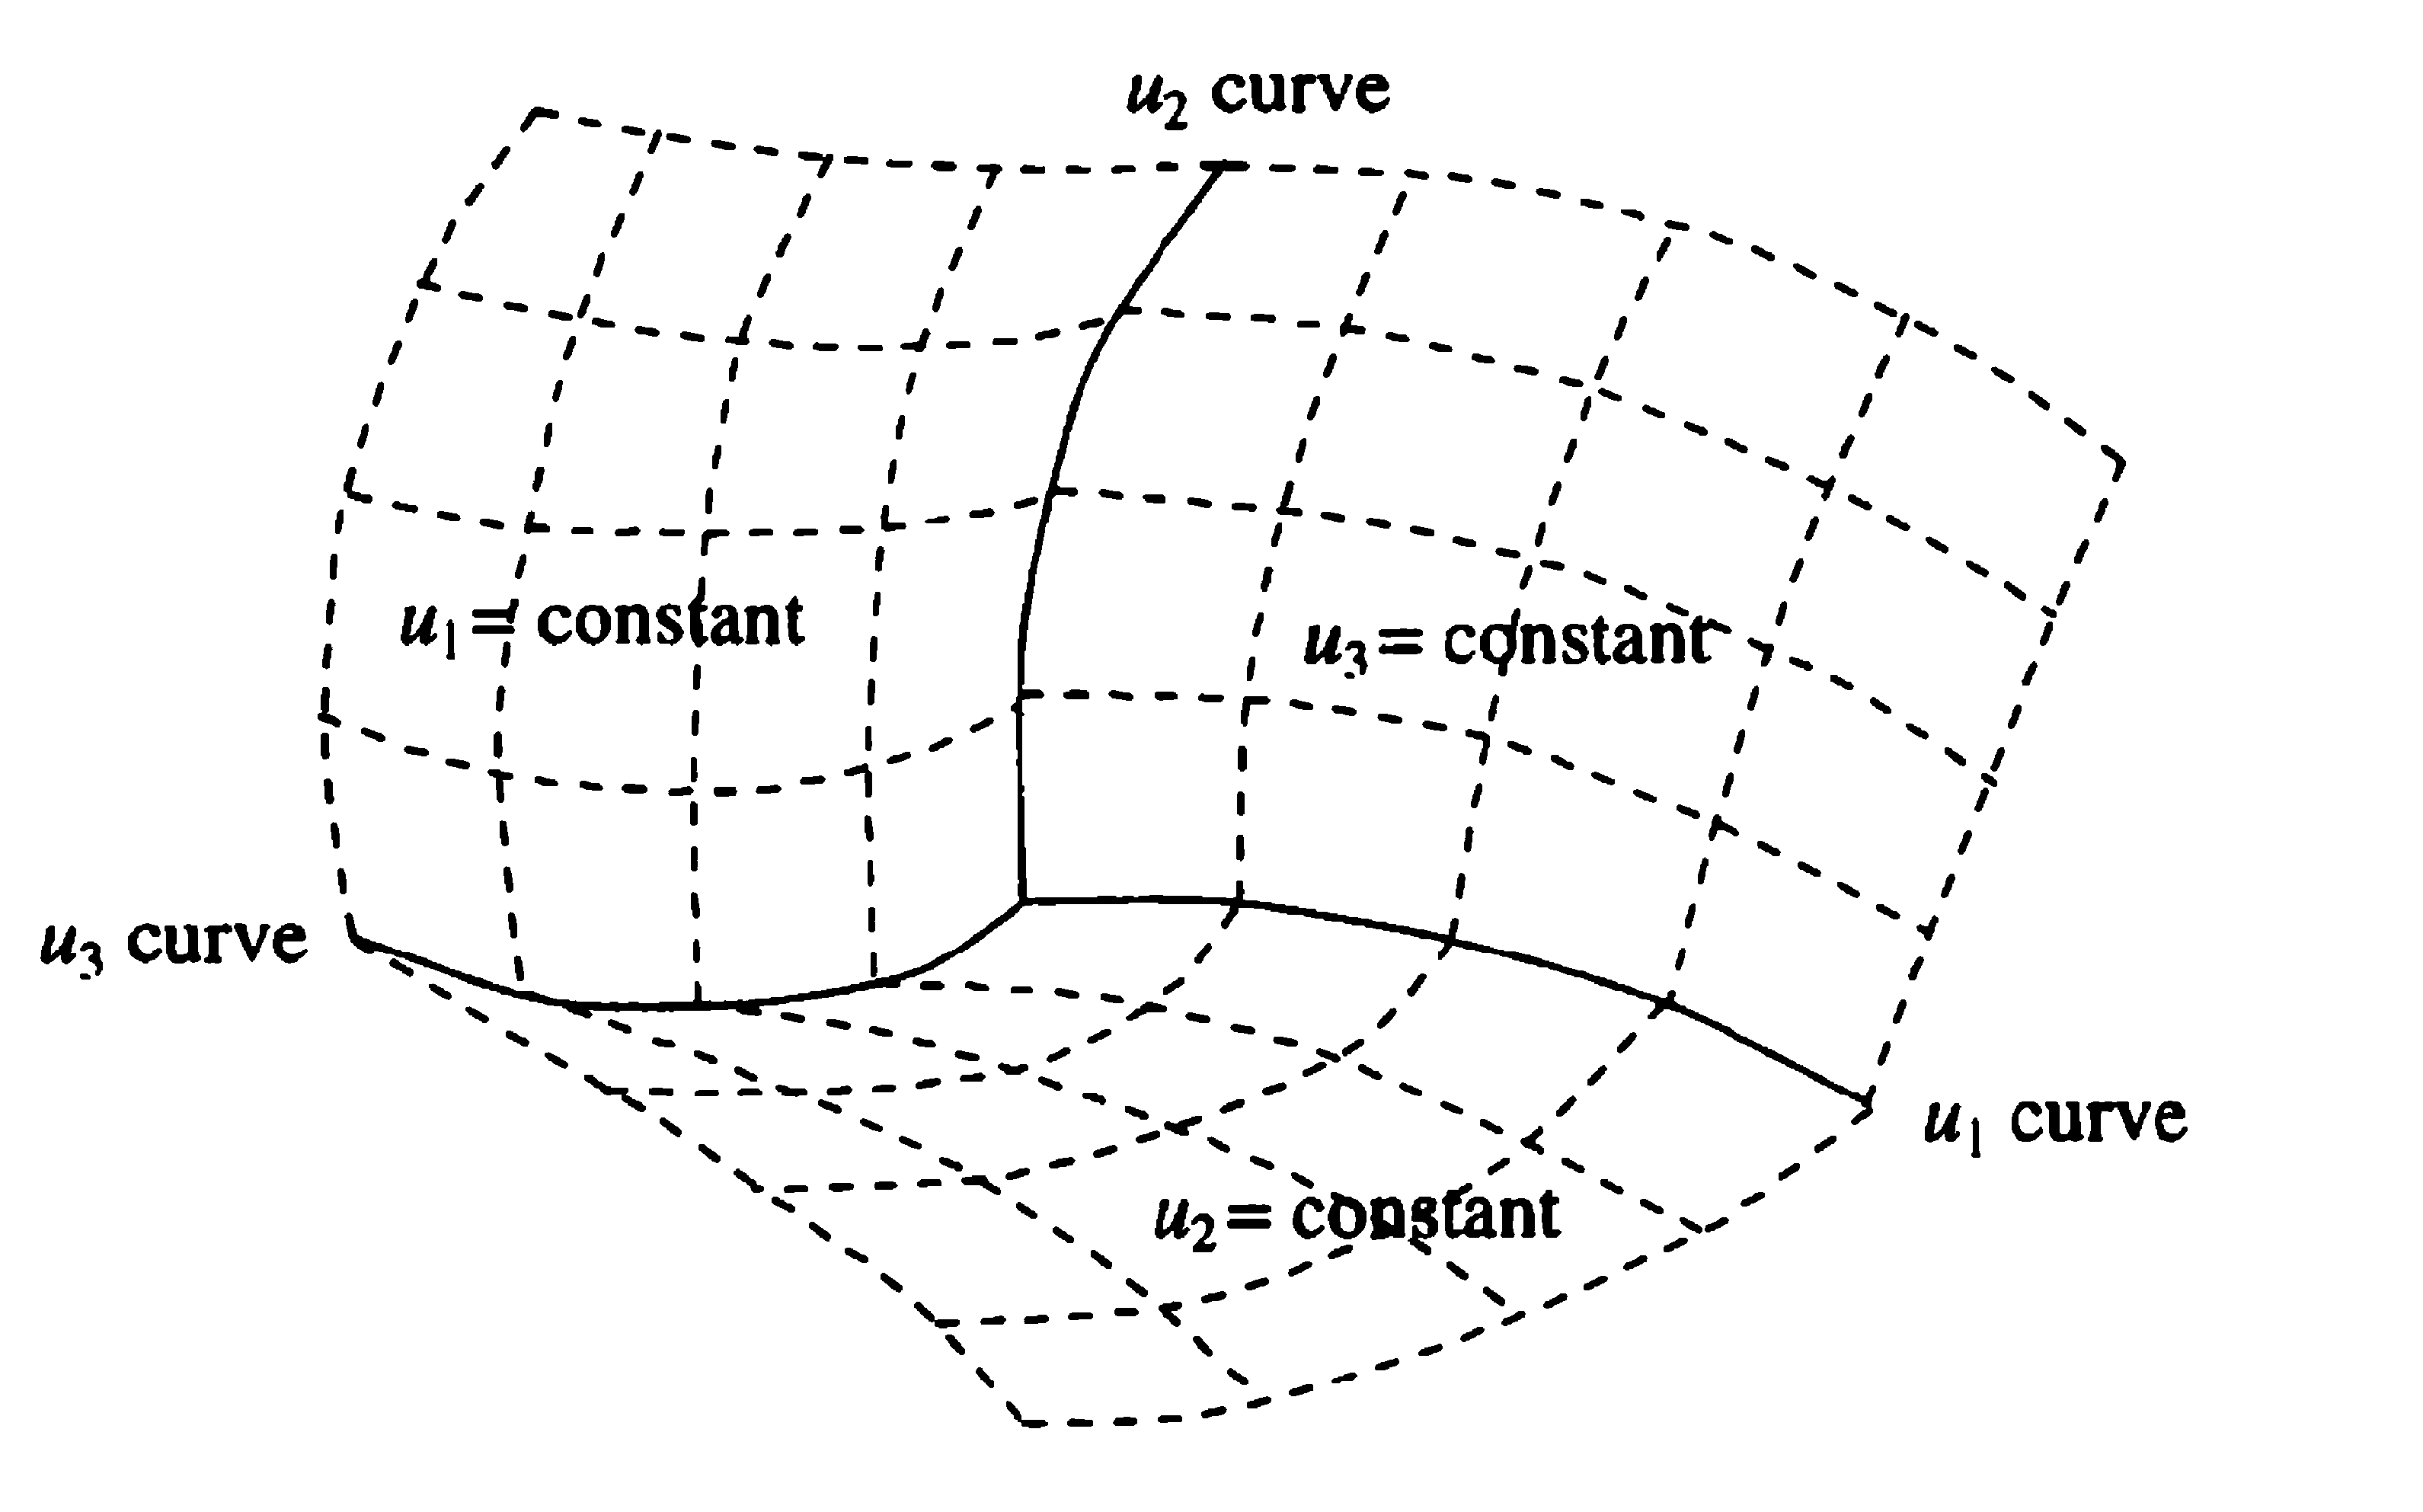
\includegraphics[scale=0.26]{fig/a-1.eps}
    \caption{曲线坐标系}
\end{figure}

特别的, 如果空间中每一个交点处坐标曲线的切线两两垂直, 那么我们称为\textbf{正交曲线坐标系}, 我们后面对于曲线坐标系中的梯度、旋度和散度的表达都是值正交曲线
坐标系的, 常见的诸如极坐标系, 球坐标系和柱坐标系都属于正交曲线坐标系。

现在我们要去看看曲线坐标系里面的微分和直角坐标系之间的关系, 我们总是倾向于去讨论局部的特征, 而且那些梯度散度的定义也是在一个无穷小下定义的。下面的讨论中, 我
们都假设坐标曲面为$$u_1(x_1,x_2,x_3)=u_1,u_2(x_1,x_2,x_3)=u_2,u_3(x_1,x_2,x_3)=u_3$$相应的, 每一点的坐标可以写成$(u_1,u_2,u_3)$。

现在我们假设直角坐标系中有一个微小的位移$\bm{dx}=(dx_1,dx_2,dx_3)$, 注意, 我们谈论两个坐标系, 他们之间一定是同坯的, 也就是说一定对应一个曲线坐标到直线坐标的
变换$$x_1(u_1,u_2,u_3)=0,x_2(u_1,u_2,u_3)=0,x_3(u_1,u_2,u_3)=0$$这样我们便可以把位移矢量使用曲线坐标系的坐标变换微元表示为:
$$dx_i=\frac{\partial x_i}{\partial u_j}du_j,\bm{dx}=\frac{\partial \bm{x}}{\partial u_j}du_j$$注意到上式我们使用了爱因斯坦求和约定。
观察每个$du_j$前面的系数$\frac{\partial \bm{x}}{\partial u_j}$, 这是一个向量, 而且是沿着关于$u_j$的这条坐标曲线的一个切向向量。很自然的, 模仿直角坐标系, 我
们引入方向向量
\begin{define}{方向向量和拉梅系数}
    \begin{lequation}
    \boxed{
        \bm{e_j}\overset{def}{=}\frac{1}{h_j}\frac{\partial \bm{x}}{\partial u_j},h_j=\left|\frac{\partial \bm{x}}{\partial u_j} \right|
    }
\end{lequation}
\end{define}
上式中的$h_j$称为\textbf{拉梅系数}, 它定义了坐标系在局部如何伸缩, 这里要明确, $du_j$只是表示坐标的变化, 虽然在通常的欧几里得空间直角坐标系中, $dx$的变化
有明确的几何意义, 它可以直接表示位移在$x$轴方向上的投影, 但是, $du$只是一个参量的变化, 没有明确的几何意义, 拉梅系数就是一种伸缩效应, 直角坐标到曲线坐标的过程中
还有伸缩, 拉梅系数就决定了这种伸缩的大小, 决定了你坐标参量变化与实际在$u_j$的方向产生的长度变化的比例关系。
\begin{thinknote}
    这里还要说明一点, 拉梅系数和单位矢量的方向、大小
    在每一点一般都是\textbf{不同的}!, 这也就是曲线坐标系让人头疼的地方, 比如你要使用曲线坐标的导数表示速度, 你需要考虑单位矢量随着质点移动的变化, 你需要对单位矢量求导!
    (实际上方向导数不是随时间变化的, 只是每一点的方向导数不同, 而质点的坐标又随时间变化)。这恰恰也就是为何极坐标系下速度的导出式子相对麻烦。
\end{thinknote}
在正交曲线坐标系中还有下面的正交关系:$$\bm{e_i}\bm{e_j}=\delta_{ij}$$
\begin{theorem}{曲线坐标系下的微元}
    \begin{itemize}
        \item $\bm{dx}=h_1\bm{e_1}du_1+h_2\bm{e_2}du_2+h_3\bm{e_3}du_3$
        \item $dS_1=h_2h_3du_2du_3$
        \item $dV=h_1h_2h_3du_1du_2du_3$
    \end{itemize}
\end{theorem}
上式中$dS$和$dV$就是指以坐标曲面/曲线去分割整个空间得到的面积微元和体积微元。也就是常常我们使用坐标变换求体积分或者是面积分要做的第一件事情, 求微元, 而且由于我们
使用的求积分的方法, 要求的微元一定是要按照坐标曲线去分割的。这里你要是使用Jacobi行列式去求, 结果相同, 实际上$J=\frac{\partial \bm{x}}{\partial u_1}\cdot
\frac{\partial \bm{x}}{\partial u_2}\times\frac{\partial \bm{x}}{\partial u_3}$, Jacobi行列式的实质是这三个向量的混合积。我认为使用这个方法更能体现出几何实质(\ref{曲线坐标微元})。
按照坐标曲线去划分出微元然后再使用梯度、旋度和散度的定义(梯度使用定义式$df=\nabla f \cdot \bm{ds}$), 可以很容易地推出下面的式子:
\begin{theorem}{梯度、旋度和散度在曲线坐标系下的表现形式}
    \begin{itemize}
        \item $\nabla f = \frac{1}{h_1}\frac{\partial f}{\partial u_1}\bm{e_1}+\frac{1}{h_2}\frac{\partial f}{\partial u_2}\bm{e_2}+\frac{1}{h_3}\frac{\partial f}{\partial u_3}\bm{e_3}$
        \item $\nabla \cdot \bm{v} = \frac{1}{h_1h_2h_3}\left(\frac{\partial}{\partial u_1}(v_1h_2h_3)+\frac{\partial}{\partial u_2}(v_2h_3h_1)+\frac{\partial}{\partial u_3}(v_3h_1h_2)\right)$
        \item $\nabla^2 f = \frac{1}{h_1h_2h_3}\left[\frac{\partial}{\partial u_1}\left(\frac{h_2h_3}{h_1}\frac{\partial f}{\partial u_1}\right)
               +\frac{\partial}{\partial u_2}\left(\frac{h_3h_1}{h_2}\frac{\partial f}{\partial u_2}\right)
               +\frac{\partial}{\partial u_3}\left(\frac{h_1h_2}{h_3}\frac{\partial f}{\partial u_3}\right)\right]$
        \item 
        \begin{math}
            \displaystyle
            \nabla \times \bm{v}=
            \frac{1}{h_1h_2h_3} 
            \begin{vmatrix}
            h_1\bm{e_1}&  h_2\bm{e_2} & h_3\bm{e_2} \\
            \frac{\partial }{\partial u_1} & \frac{\partial }{\partial u_2} & \frac{\partial }{\partial u_3}\\
            h_1v_1 & h_2v_2 & h_3v_3
            \end{vmatrix}
        \end{math}
    \end{itemize}
\end{theorem}
\begin{thinknote}
    下面来推导一下最后一个式子:
    $$\nabla \times \bm{u} \cdot \bm{\hat{n}} \overset{def}{=}\lim_{\delta S \to 0}\frac{1}{\delta S} \oint_{\delta C} \bm{u} \cdot \bm{dr}$$

    考虑一个在$u_3$坐标曲面上的小矩形(\ref{旋度计算}), 也即$u_1$和$u_2$变化时产生的几何微元, 利用这个矩形去求旋度在$e_3$方向上的分量大小。

    首先计算环量, 注意到$\bm{v}$的分量的方向以及积分方向的关系, 不难得到左右两边积分为
    $$[v_2h_2](u_1+\frac{du_1}{2},u_2,u_3)du_2-[v_2h_2](u_1-\frac{du_1}{2},u_2,u_3))du_2$$
    注意, 这里$v_2h_2$是随着坐标而变化的, 将$v_2h_2$整体看成是一个函数, 只有$u_1$变了, 泰勒展开进行一阶近似得到
    $$\frac{1}{h_1h_2}\frac{\partial}{\partial u_1}(v_2h_2)$$
    类似的方法可以计算出上下边的积分为:
    $$-\frac{1}{h_1h_2}\frac{\partial}{\partial u_2}(v_1h_1)$$
    注意到我们这样计算最后得到的是垂直于积分曲线围成的曲面的法向方向旋度分量, 也即:
    $$\bm{e_3}\cdot\nabla\times\bm{v}=\frac{1}{h_1h_2}\left(\frac{\partial}{\partial u_1}(v_2h_2)-\frac{\partial}{\partial u_2}(v_1h_1)\right)$$
    对每一个方向都进行计算后便可以得到上面的公式
\end{thinknote}
物理量比如速度表达式的推导只需要将时间$t$这个参数引入就行了。比如:$$\bm{v}=\frac{\bm{dx}}{dt}=h_1\dot{u_1}\bm{e_1}+h_2\dot{u_2}\bm{e_2}+h_3\dot{u_3}\bm{e_3}$$
要求加速度, 将上式对时间再求一阶导数即可。在这里重新说明一下, 这个单位矢量本身不是随时间变化的, 是随空间坐标变化的, 但是质点运动时, 空间坐标显含时间, 所以相当于是
质点自身来看, 单位矢量隐含时间项。
\begin{figure}[htbp]
    \centering
    \label{旋度计算}
    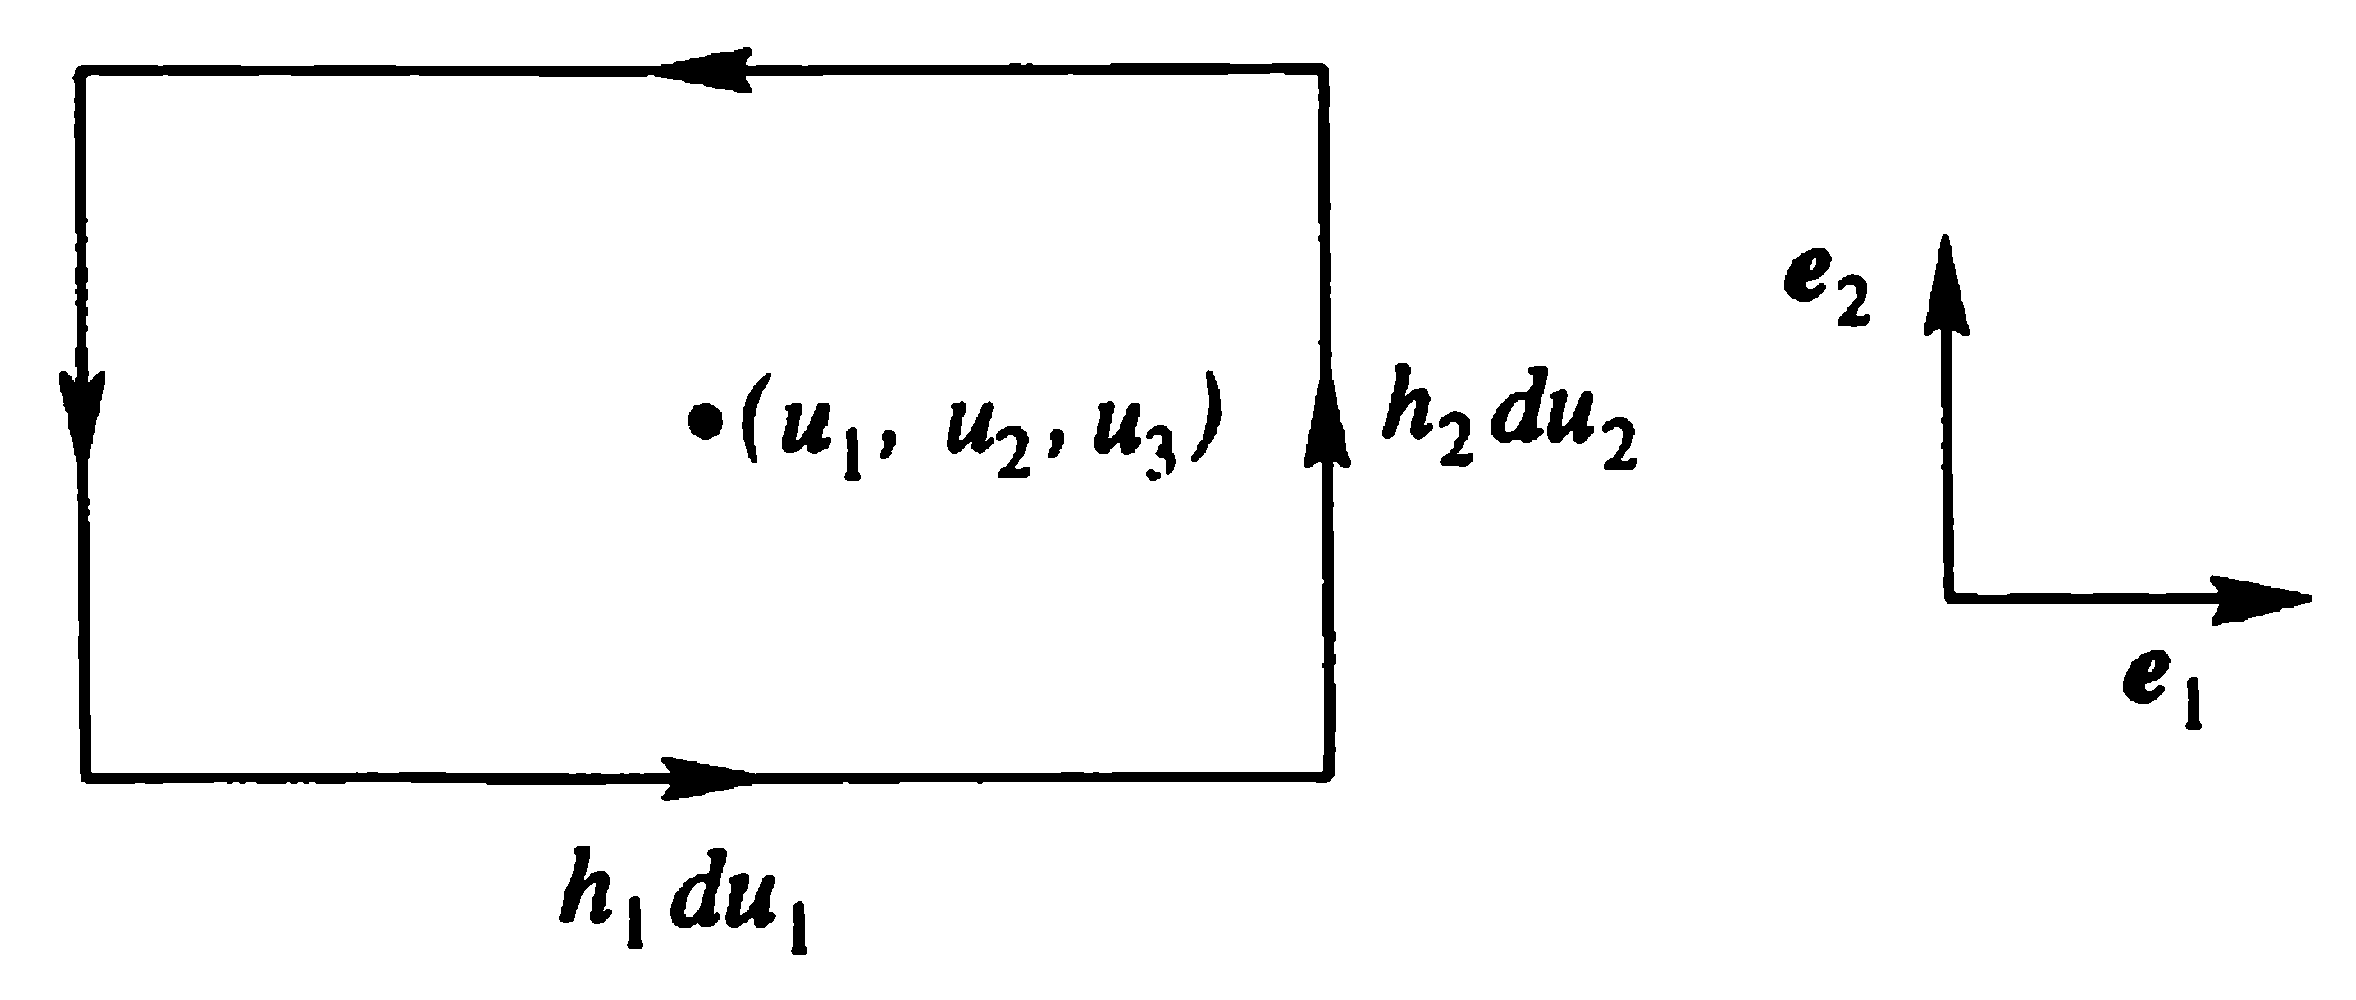
\includegraphics[scale=0.3]{fig/a-3.eps}
    \caption{计算旋度}
\end{figure}
\begin{figure}[htbp]
    \centering
    \label{曲线坐标微元}
    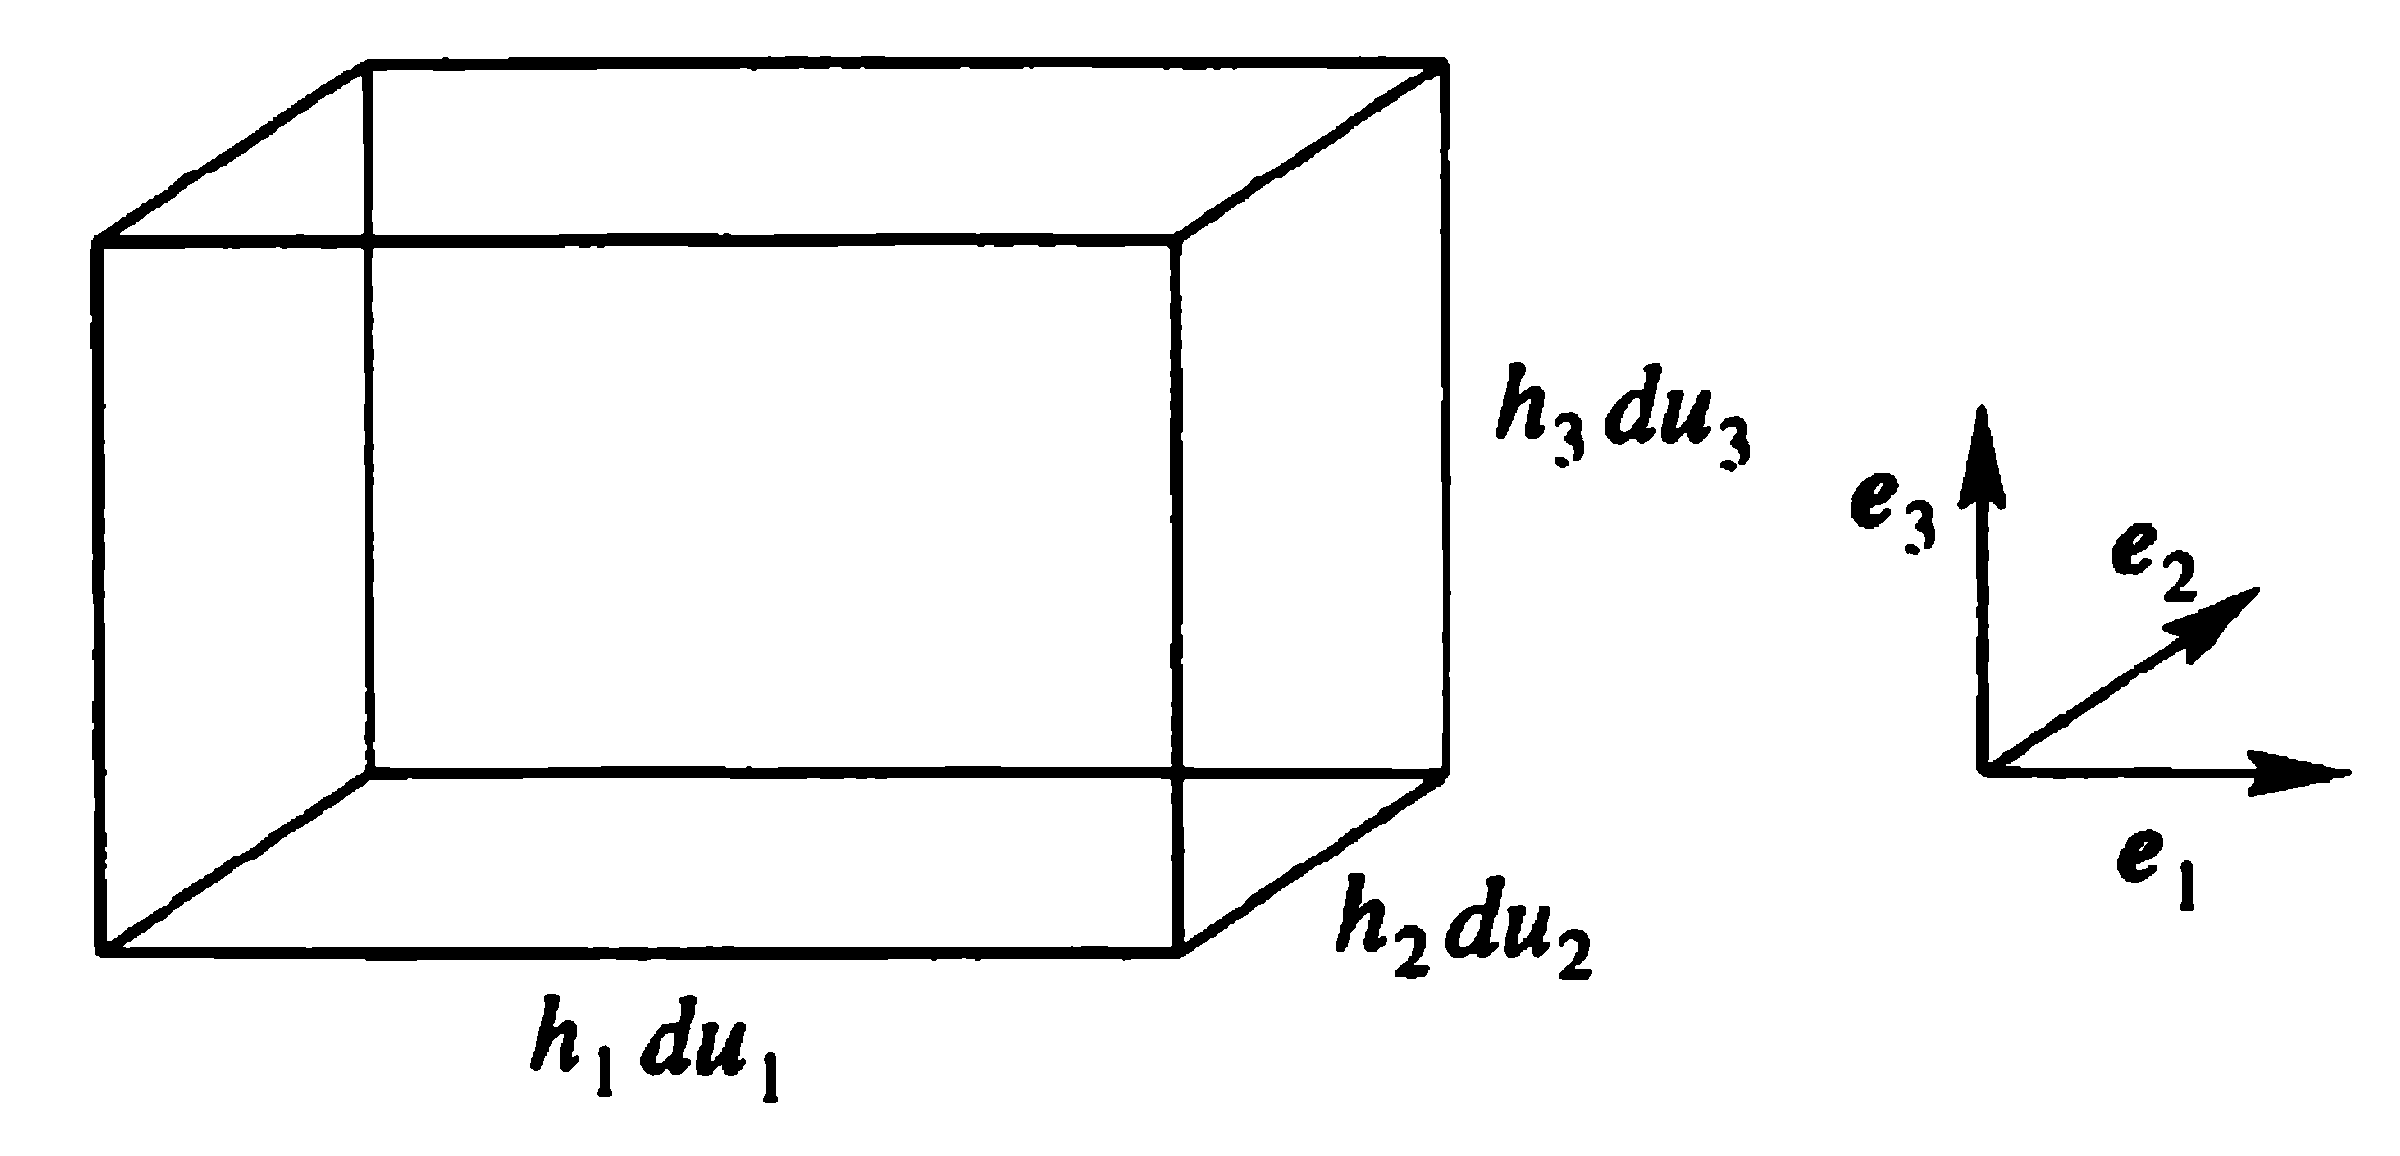
\includegraphics[scale=0.26]{fig/a-2.eps}
    \caption{曲线坐标系的局部就可以看成一个小(不再是直角坐标里面的正方体了), 图中也标出了参数微元和实际位移量的比例关系}
\end{figure}
\section{曲线积分和曲面积分}
在继续之前我想重新对这部分内容稍微探讨一下, 读者或多或少在通常的微积分课本中已经学到过这两个概念, 通常的微积分课本包括广受赞誉的菲赫金哥尔茨的微积分学教程, 讨论相对于原先的入射波
这部分内容时, 基本上都还是使用投影方法去划归为通常的积分来进行计算。 其实, 笔者认为, 理解这一部分内容的最好的方法就是全部划归为参数形式去理解, 而书本上提到的
投影法, 就是直接将直角坐标系中的三个坐标作为参数来计算, 这样选取参量更加具有几何意义, 可以在一定程度上方便随后参量的变化范围的确定, 从物理系学生的角度上看, 我
觉得从一开始就使用参数形式即向量运算的角度去理解这几个概念是有好处的。这一部分的内容主要参考的就是我自身上课时整理的高数笔记。

重点不是去记住计算方法本身, 而是去理解, 曲线积分和曲面积分是对向量场的积分, 前面的积分都是对标量场的积分, 物理学中涉及到大量的向量场, 所以完全有必要在矢量分析
这块重提一下这两个概念。
\subsection*{曲线积分}
曲线积分分为两类, 一个对弧长, 一个对坐标, 实际上我们利用向量式写出来就变成了下面的形式:
\begin{align}
    \int_L \bm{f(\bm{r})}|\bm{dr}|\tag{a}\\
    \int_L \bm{A}\cdot\bm{dr}\tag{b}
\end{align}

直接使用向量的运算法则去理解, 我们将曲线用参数形式表示, 而且重要的是用参数表示出每一点的\uwave{矢径}。即, 我们改用$\bm{r}=\bm{r}(t)$去描述曲线$L$, 自然
的, 我们就可以对这个向量函数求导得到每一小段有向弧矢量, 使用参数$t$表示。$\bm{dr}=\bm{r}^\prime(t)dt$, 注意, 得到的是一个向量, 我们直接将得到的微分式子
直接按照曲线积分的向量形式代入便可以将其转化为通常的一元积分。

但是上面的代入过程中要注意参量的上下限, 对于第一型, 从定义可以知道是对弧长的积分, 所以始终是积分上限大于下限; 对于第二型, 要注意积分的方向, $t$从积分下限
走到积分上限, 对应的, 曲线要从起点走到终点, 可以很简单的验证$\bm{r}^\prime(t)$的方向始终是$t$增大时曲线的走向, 那么当积分上限小于积分下限时, 也就对应了$dt<0$
积分方向刚好反向。

利用向量观点之后, 就可以理解更广义的曲线积分, 比如:
\begin{equation}
    \int_L \bm{A}\times\bm{dr}\tag{c}
\end{equation}
计算方法是一样的, 写出曲线的向量表示形式后求出$\bm{dr}$, 直接代入定义式计算即可。
\subsection*{曲面积分}
到曲面积分这里, 通常的教科书就几乎没有使用向量的语言去描述了。实际上, 这部分相比于曲线积分只是多了一个参量, 曲面$S$需要表示为$\bm{r}=\bm{r}(u,v)$的形式。
那么曲线积分使用向量的表示可以进一步变为:
\begin{align}
    \iint_S f(\bm{r})|\bm{dS}|\\
    \iint_S \bm{A}\cdot\bm{dS}
\end{align}

求曲面积分的时候, 我们使用$u,v$的一系列等值线去分割曲面$S$, 局部来看就是一系列小平行四边形, 有了前面曲线坐标系的观点, 我们可以得出局部的小平行四边形的面积元
矢量可以使用叉乘形式表达为:
$$\bm{dS}=\pm\frac{\partial \bm{r}}{\partial u}\times\frac{\partial \bm{r}}{\partial v}dudv$$
前面的正负号选取要根据实际积分中规定的曲面方向确定。

同我们前面做的一样, 下一步直接代入就可以得到解。这里我们说明一下, 面积元矢量前面的正负号你可以认为是$du,dv$的正负号决定的, 就跟我们前面的曲线积分一样, 你
可以计算前就通过曲面的法向量方向选取定好正负号(那两个切向量都取$u,v$增大时曲面切线方向), 然后计算时积分上限就始终大于积分下限, 第二种做法就是积分时首先不去
确定这个面元前面取正还是取负, 而是在$u,v$的上下限选取中体现出曲面的法向量的方向。 我更偏爱第一种方式, 曲面相较于曲线使用第二种方式可能有点复杂。利用这个思路
再去看书上在转换时产生的因子$\sqrt{1+z_x^2+z_y^2}$也就有了新一点的体会。

当然, 第二型曲面积分, 也可以将被积向量场在曲面法向量方向上投影后转化为第一类曲线积分求解, 这里不多叙述了。这部分的内容更深的讲解应自行翻阅\uwave{微分几何}
书籍。
\section{直角坐标里的张量}
在探讨什么是张量之前, 我们需要重新定义一下什么是标量和矢量, 下面的讨论都是在直角坐标系下的。

考虑坐标系的旋转, 空间中某一点在两个坐标系中的坐标$\bm{X'}$和$\bm{X}$由一个过渡矩阵$\bm{L}$联系起来。这个矩阵就是我们所熟知的\uwave{转动矩阵}, 是一个正交
矩阵
\begin{lequation}
    \label{eq:A.7}
    \boxed{
        \bm{L}=
        \begin{pmatrix}
           \cos\theta & \sin\theta \\
           -\sin\theta& \cos\theta
        \end{pmatrix}
    }
\end{lequation}
\begin{center}
    \begin{math}
        \displaystyle
        \begin{pmatrix}
            x_1' \\
            x_2'
        \end{pmatrix}
        =\bm{L}
        \begin{pmatrix}
            x_1\\
            x_2
        \end{pmatrix}
        \qquad
        \bm{L}\bm{L^T}=\bm{L^T}\bm{L}=\bm{I}
        \qquad
        \left|\bm{L}\right|=1
    \end{math}
\end{center}
上面的后两个式子是正交矩阵自身的性质, 第一式使用求和约定写成
\begin{center}
    \begin{math}
        \displaystyle
        x_i'=L_{ij}x_j\qquad
        x_i =L_{ji}x_j'
    \end{math}
\end{center}
注意用到了$\bm{L^T}=\bm{L^{-1}}$这个条件。对于更高纬度的欧式空间, 每个基向量若还是有正交关系, 即$\bm{e_i}\cdot\bm{e_j}=\delta_{ij}$。旋转变换是保长
变换, 我们仍旧可以使用两个坐标基向量之间的确定转换矩阵为
\begin{lequation}
    \boxed{
        L_{ij}=\bm{e_i'}\cdot\bm{e_j}
    }
\end{lequation}
这个矩阵还是一个正交矩阵, 但是注意, $L^TL=I$不能说明$\left|L\right|=\pm 1$, 行列式的值取$1$才表示\textbf{旋转变换}, 取$-1$表示\textbf{反射变换}。
这个矩阵还是一个实矩阵, 是一个\uwave{等距同构}算子的矩阵, 线性代数中可以证明实内积空间上的等距同构\footnote[1]{回忆一下等距同构一定是正规的}的矩阵有下面性质
\begin{theorem}{实内积空间上的等距同构}
    如果$S$是实内积空间上的某个等距同构, 那么它关于某个规范正交基的矩阵一定是一个分块对角阵, 而且每个块中的元素是$\pm 1$或者
    \begin{center}
        \begin{math}
            \displaystyle
            \begin{pmatrix}
                \cos\theta & \sin\theta \\
                -\sin\theta& \cos\theta
            \end{pmatrix}
        \end{math}
    \end{center}
\end{theorem}
显然, 我们这里的等距同构就是一个$R^n$上的旋转变换, $L$就是它的矩阵表示。下面还有关于$L$的两个等式:
\begin{lequation}
    \frac{\partial x_i'}{\partial x_j}=L_{ij} \qquad \text{and} \qquad \frac{\partial x_i}{\partial x_j'}=L_{ji}
\end{lequation}
\begin{define}{标量和矢量}
    \begin{itemize}
        \item 
        $\bm{v}$是一个矢量, 当且仅当在坐标系进行旋转变换时, 它在两个坐标系下的分量之间的变换与$\bm{L_{ij}}$一致, 也就是说它的变换和点的变换时一致的:$$v_i'=L_{ij}v_j$$
        \item 标量定义为在坐标系的旋转变换下,值始终不变的量$$s'=s$$
    \end{itemize}
\end{define}
我们抛弃了原先矢量的定义, 一个有大小有方向的量, 取而代之的是一个更加抽象化的描述, 也更加精确, 同时也为我们将定义扩展到张量上带来了便利, 使用定义我们可以证明
两个矢量的点乘是标量。
\begin{thinknote}
    对于矢量$\bm{a}$和$\bm{b}$我们有$$a_i'=L_{ij}a_j,b_i'=L{ij}b_j$$那么$s=\bm{a}\cdot\bm{b}=a_ib_i$, 换到另一个参考系后, 点乘的定义还是不变有
    \begin{center}
        \begin{math}
            s'=(\bm{a}\cdot\bm{b})'=a_i'b_i'=L_{ij}a_jL_{ik}b_k=L_{ij}L_{ik}a_jb_k=\delta_{jk}a_jb_k=a_kb_k=s
        \end{math}
    \end{center}
    这就证明了$\bm{a}\cdot\bm{b}$是标量。 
\end{thinknote}
这也是证明一个量是否是矢量或标量的一般方法
\footnote[1]{注意到上面的证明利用了
    $$\bm{L}\bm{L^T}=\bm{I}\Rightarrow L_{ij}L^T_{jk}=\delta_{ik} \xLongrightarrow{L^T_{jk}=L_{kj}} L_{ij}L_{kj}=\delta_{ik}$$
    使用$\bm{L^T}\bm{L}=\bm{I}$可以导出我们证明需要的等式}
, 考虑它的基本得到方法, 然后再两个坐标系下的表示, 最后考虑其分量随
坐标变换的变换关系。

下面将定义推广到张量, 我们前面接触的矢量, 只有一个自由指标, 但是张量却有多个自由指标。
\begin{define}{张量}
    $T$是一个\uwave{二阶张量}, iff.坐标变换时满足$$T'_{ij}=L_{ik}L_{jm}T_{km}$$同理, 三阶张量就是坐标变换时满足下面关系的量$$P'_{ijk}=L_{ip}L_{jq}L_{kr}P_{pqr}$$
    我们也常常将标量称为\uwave{零阶张量}, 矢量称为\uwave{一阶张量}。
\end{define}
前面提到的$\delta_{ij},\epsilon_{ijk}$就是张量的例子, 证明方法和证明一个量是否是矢量类似, 下面介绍一个很有用的定理去判断一个量是不是张量, 在物理定律中可以用
它来迅速发现一个量的张量本质。
\begin{theorem}{商法则(Quotient Rule)}
    $$a_i=T_{ij}b_j$$
    如果对于坐标系的任何一个变换, 对于任何一个矢量$\bm{b}$, 使用上面式子计算出来的$\bm{a}$都是一个矢量, 那么$T$是一个张量。
    
    这个定理还可以推广, 如果对于任意一个$n$阶张量$B$和任意坐标变换使用下面的式子得到的$A$总是个$m$阶张量, 那么$T$一定是一个$m+n$阶张量。
    \begin{center}
        \begin{math}
            \displaystyle
            A_{\underbrace{ijk\ldots}_{m}}=T_{\underbrace{ijk\ldots\alpha\beta\gamma\ldots}_{m+n}}B_{\underbrace{\alpha\beta\gamma\ldots}_{n}}
        \end{math}
    \end{center}
\end{theorem}
直角坐标系里, 我们可以使用一个n-by-1的矩阵表示一个向量, 而对于一个二阶张量我们需要一个二维的n-by-n矩阵去描述, 三阶张量需要使用一个立体的矩阵去描述, 到了
更高维就很难去想象这样一个“矩阵”了。注意, 张量、矢量本身是不随坐标系变换改变的, 只是分量在不同坐标系下可能不同, 所以不同坐标系下描述它的矩阵可能有点差别。

\begin{define}{对称张量和反对称张量}
    这个的定义和对称矩阵的定义非常相似 
    \begin{itemize}
        \item \textbf{对称张量}: 任意两个下标对换后得到的两个分量始终相等, 如$T_{ij}\equiv T_{ji}$
        \item \textbf{反对称张量}: 任意两个下标对换后得到的两个分量始终互为相反数, 如$T_{ij}\equiv -T_{ji}$
    \end{itemize}
    $\delta_{ij}$是对称张量, $\epsilon_{ijk}$是反对称张量, 所以$ijk$中任何两个值相等时$\epsilon=0$。

    虽然不同的坐标系下张量的分量不同, 但张量对称性质不随坐标系的变换而变化。
\end{define}
\begin{define}{各向同性张量}
    如果一个张量的每一个分量在不同的坐标系下都相同, 那么这个张量称为\textbf{各向同性张量}。
\end{define}
各向同性张量事实上非常少可以证明各向同性张量只可能是下面的形式:
\begin{proposition}{n阶各向同性张量}
    \begin{itemize}
        \item 0-order: 都是各向同性的
        \item 1-order: 只有$\bm{0}$是各向同性的
        \item 2-order: 只有$a_{ij}=\lambda \delta_{ij}$是各向同性的
        \item 3-order: 只有$a_{ijk}=\lambda \epsilon_{ijk}$是各向同性的
        \item 4-order: 只有$a_{ijkl}=\lambda\delta_{ij}\delta_{kl}+\mu\delta_{ik}\delta_{jl}+\nu\delta_{il}\delta_{jk}$是各向同性的
    \end{itemize}
\end{proposition}
在物理学中, 张量的出现总是伴随着两个矢量, 使用商法则, 我们就可以判断一个量是张量, 正是张量的存在才让两个矢量之间的关系变得复杂起来。
\subsubsection*{电导率张量}
我们先回顾一下欧姆定律的微分形式$$\bm{j}=\sigma\bm{E}$$初学电磁学时会简单的认为$\bm{j}$和$\bm{E}$的方向相同, 只是在所谓的长度上有一个伸缩关系。实则不然
在一般的介质中, 这两个矢量是不平行的, 我们考虑一个极端情况
\begin{figure}[htbp]
    \centering
    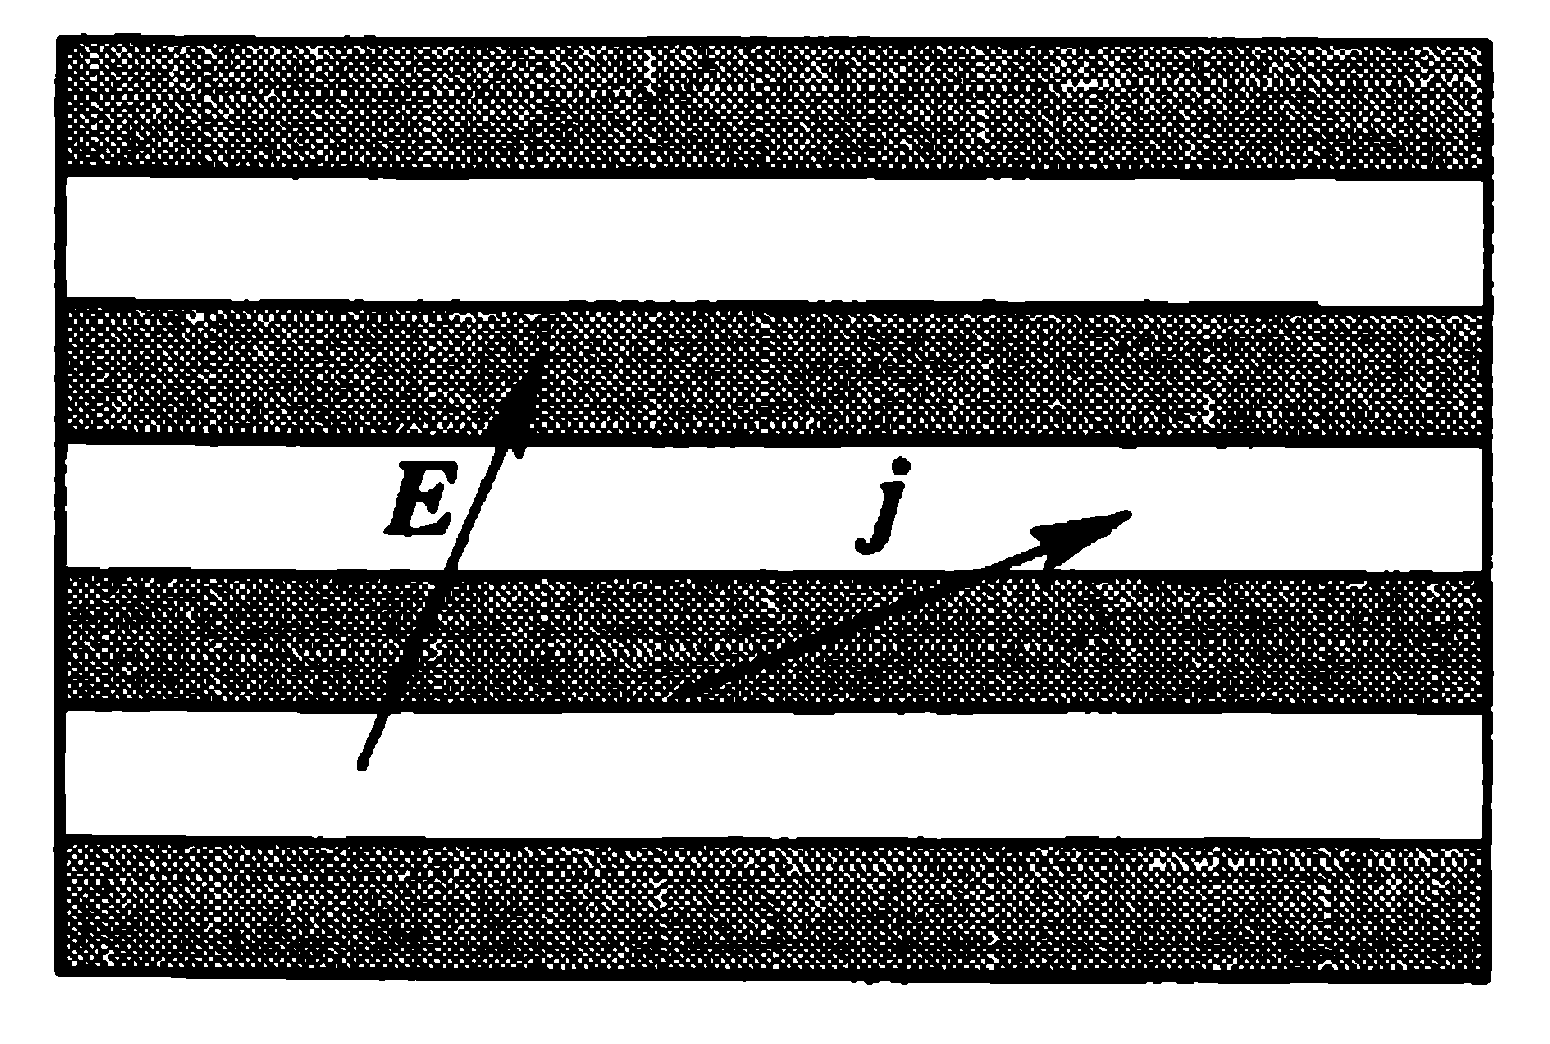
\includegraphics[scale=0.3]{fig/a-4.eps}
    \caption{电导率张量}
\end{figure}
这个介质是由两种不同的介质构成的,不再和我们一般的介质一样是各向同性的, 在每一层介质中, 和我们之前学的确实是一致的, 但是当你考虑边界面处$\bm{j}$和$\bm{E}$的
关系时, 会有很大的不同。 我们假设白色的介质电导率很低,就像是绝缘体一样, 而灰色的介质导电率很高, 是一个良导体。这个时候显然电流更容易沿着边界面流动, 而不是
穿过界面\footnote[1]{你可以想象一堵墙阻挡你, 无论别人用多大的力气推你, 你也只能沿着墙走},所以就会导致两个矢量方向不同, 这个时候如果$\sigma$是一个标量肯定
不符合要求, 这个时候就要求$\sigma$是一个张量了, 而且$$j_i=\sigma_{ik}E_k$$在我们讨论的这个情况下, 这个张量可以使用矩阵描述为:
\begin{center}
    \begin{math}
        \displaystyle
        \sigma=
        \begin{pmatrix}
            \sigma_0&0&0\\
            0&\sigma_0&0\\
            0&0&0
        \end{pmatrix}
    \end{math}
\end{center}
其中$x$轴平行于分界面, $y$轴垂直于分界面, $z$轴垂直于纸面。

当我们讨论的介质各向同性, 每个地方的电导率相等时, 这个张量和我们前面定义的各向同性张量是一样的, 分量不随坐标系变换而变化。那么$\sigma_{ij}=\sigma_0\delta_{ij}$
$$j_i=\sigma_{ik}E_k=\sigma_0\delta_{ik}E_k=\sigma E_i\Rightarrow\bm{j}=\sigma_0bm{E}$$张量退化为了我们熟知的标量。
\subsubsection*{惯量张量}
初学力学时, 一直在强调, 刚体的角动量和角速度一般情况下方向是不同的, 我们刚体平行平面运动中所列的转动方程实际上是列的投影式$M_z=I_{zz}\frac{d\omega_z}{dt}$(其中转轴就是
$z$轴, 角速度方向和$z$轴方向相同), 这也说明转动惯量也应该是一个张量, 只是我们在计算的都是均匀的几何体, 具有各向同性, 惯量张量退化为一个标量。惯量张量也可以
表示为一个矩阵, 对角线元素是转动惯量, 非对角线元素叫做惯量积。Feynman讲义第一卷中也讨论了这个问题, 就是因为几何体的不均匀性才导致了转动惯量是张量, 这一点
在刚体做定轴转动是尤为明显。

我们下面计算一个刚体绕某个基点以$\Omega$角速度转动时的角动量矢量的第$i$个分量:
\begin{center}
    \begin{equation*}
        \displaystyle
        \begin{split}
            L_i&=\iiint_V \rho(\bm{r}\times\bm{v})_idV\\
               &=\iiint_V \rho(\bm{r}\times\left(\bm{\Omega}\times\bm{r}\right))_idV\\
               &=\iiint_V \rho\left(r^2\Omega_i-\left(\bm{r}\cdot\bm{\Omega}\right)r_i\right)dV \qquad\qquad\text{(Lagrange恒等式)}\\
               &=\iiint_V \rho\left(r^2\delta_{ij}\Omega_j-r_j\Omega_jr_i\right)dV\\
               &=\iiint_V \rho\left(r^2\delta_{ij}-r_jr_i\right)\Omega_jdV\\
        \end{split}
    \end{equation*}
\end{center}    
定义惯量张量$$I_{ij}=\iiint_V \rho\left(r^2\delta_{ij}-r_jr_i\right)$$
那么角动量和角速度之间的关系又下式给定:
$$L_i=I_{ij}\Omega_j$$
再从角速度和角动量的矢量性质, 由商法则可以判断$I$是二阶张量, 也正是由于它的张量性质才有了角动量和角速度方向的不同。

\section{分部积分法}
在单变量微积分中学到的分部积分(Integration by Parts)公式:
\begin{equation}
    \int_a^buv^\prime dx=\left. {{uv}} \right|_a^b-\int_a^bu^\prime v dx
\end{equation}
是计算积分的强有力的武器, 但是我们在量子力学中遇到的大多数都不是单变量的情况, 所以有必要将上述分部积分法扩展到更高维的情形中去。

下面假设$u$是任意一个标量场, $\mathbf{V}$是任意一个向量场。利用散度的计算公式有:
\begin{equation}
    \label{eq:A.11}
    \nabla\cdot\left(u\mathbf{V}\right)=u\nabla\cdot\mathbf{V}+\nabla u\cdot\mathbf{V}
\end{equation}
另外设$\Omega$是$\mathbbm{R}^n$中的一个可积区域, 我们现在对\ref{eq:A.11}两边同时积分:
\begin{equation}
    \label{eq:A.12}
    \int_\Omega \nabla\cdot\left(u\mathbf{V}\right)d\Omega =\int_\Omega u\nabla\cdot\mathbf{V} d\Omega +\int_\Omega\nabla u\cdot\mathbf{V}d\Omega
\end{equation}
根据高斯定理\footnote{我们并没有对高维空间中的高斯定理进行一般的证明, 姑且就先承认它在高维空间的推广是显然的。},\ref{eq:A.12}左边应该等于:
\[\text{l.h.s}=\oint_\partial\Omega u \mathbf{V}\cdot d\mathbf{S}\]
对比一下单变量的分部积分公式, 我们便可将\ref{eq:A.12}重写为:
\begin{equation}
    \label{eq:int-by-parts}
    \boxed{
        \int_\Omega u\nabla\cdot\mathbf{V} d\Omega=\oint_\partial\Omega u \mathbf{V}\cdot d\mathbf{S}-\int_\Omega\nabla u\cdot\mathbf{V}d\Omega
    }
\end{equation}
数学上还有一些具体的注意事项我们物理这边就不太在乎了, 实际上这个公式和一维情况是及其相似的, 我们用这个公式的时候很多情况下都是边界项为$0$, 即
\[\int_\Omega u\nabla\cdot\mathbf{V} d\Omega=-\int_\Omega\nabla u\cdot\mathbf{V}d\Omega\]
\subsection*{Green's first identity}
下面取向量场\footnote{$\mathbf{e}_i$是单位向量}$\mathbf{U=u_1\mathbf{e}_1+u_2\mathbf{e}_2+\cdots+u_n\mathbf{e}_n}$, 以及$\mathbf{V}=v\mathbf{e}_1+v\mathbf{e}_2+\cdots+v\mathbf{e}_n$. 我们现在试图去
求\footnote{已使用爱因斯坦求和约定}:
\[
    \int_\Omega u_i\frac{\partial v}{\partial x_i}d\Omega =\oint_{\partial\Omega} u_i v \mathbf{e}_i\cdot d\mathbf{S}-\int_\omega\frac{\partial u_i}{\partial x_i}v d\Omega
\]
上式的推导即先将积分和求和交换次序, 对于每个积分我们都认为$v\mathbf{e}_i$可以看作是只有一个分量不为0的向量场, 便可套用公式\ref{eq:int-by-parts}即可证明。
现在我们将上式写成向量形式:
\begin{equation}
    \int_{\Omega} \mathbf{U} \cdot \nabla v d \Omega=\oint_{\partial\Omega} v \mathbf{U} \cdot d\mathbf{S}-\int_{\Omega} v \nabla \cdot \mathbf{U} d \Omega
\end{equation}
进一步, 如果$\mathbf{U}$可以写成$\mathbf{\nabla u}$的形式, 那么我们便得到了格林第一恒等式:
\begin{equation}
    \int_{\Omega} \nabla u \cdot \nabla v d \Omega=\oint_{\partial\Omega} v \nabla u \cdot  d\mathbf{S}-\int_{\Omega} v \nabla^2 u d \Omega
\end{equation}

\section{*外微分形式与斯托克斯定理(施工中)}
本节涉及到的所有公式都是下面这个及其优美结论在$\mathbbm{E}^3$中的弱化版本:\footnote{ref:《流形上的微积分》}
\begin{theorem}{Stokes Theorem}
	\begin{equation}
		\boxed{
		\int_{\partial \Omega} \omega =\int_{ \Omega} \mathrm{d}\omega 
		}
	\end{equation}
\end{theorem}
对张量场积分时有下面的重要公式:\footnote{ref:刘川《电动力学》}

balabala


\chapter{Linear Algebra}
\label{Appendix B}
这个附录主要是关于线性代数一些基本知识的回顾, 使用量子力学中的记号表示, 主要参考的是科恩塔诺基《量子力学》卷一第二章。
\section{向量空间}
在附录A中我们讨论的向量和通常物理里面所说的\uwave{有大小有方向的量}是一致的, 实际上它们是所谓欧几里得空间中的向量, 我们下面要以更抽象的思维来对待向量。
\begin{define}{向量空间}
    在数域$\mathbb{P}$上定义的向量空间$\mathscr{A}$是一个\textbf{带有数乘和加法运算的集合}, 这两种运算对于$\mathscr{A}$是\uwave{封闭的}, 且满足下面的公理。
在量子力学中, 我们使用$\left| \alpha  \right\rangle ,\left| \beta  \right\rangle $表示矢量, 后面会详细谈到这种记号。至于数域$\mathbb{P}$中的数我们一律用小写英文字母表示。
\begin{itemize}
    \item \textbf{封闭性}:
        \[\begin{array}{l}
        \left| \alpha  \right\rangle  \in \mathscr{A} \wedge \left| \beta  \right\rangle  \in \mathscr{A} \to \left| \alpha  \right\rangle  + \left| \beta  \right\rangle  \in \mathscr{A}\\
        \left| \alpha  \right\rangle  \in \mathscr{A} \to a\left| \alpha  \right\rangle  \in \mathscr{A}
        \end{array}\]
    \item \textbf{交换律}:\[\left| \alpha  \right\rangle  + \left| \beta  \right\rangle  = \left| \beta  \right\rangle  + \left| \alpha  \right\rangle \]
    \item \textbf{结合律}:\[\begin{array}{l}
        \left( {\left| \alpha  \right\rangle  + \left| \beta  \right\rangle } \right) + \left| \gamma  \right\rangle  = \left| \alpha  \right\rangle  + \left( {\left| \beta  \right\rangle  + \left| \gamma  \right\rangle } \right)\\
        \left( {ab} \right)\left| \alpha  \right\rangle  = a\left( {b\left| \alpha  \right\rangle } \right)
        \end{array}\]
    \item \textbf{分配律}:\[\begin{array}{l}
        a\left( {\left| \alpha  \right\rangle  + \left| \beta  \right\rangle } \right) = a\left| \alpha  \right\rangle  + a\left| \beta  \right\rangle \\
        \left( {a + b} \right)\left| \alpha  \right\rangle  = a\left| \alpha  \right\rangle  + b\left| \alpha  \right\rangle 
        \end{array}\]
    \item \textbf{加法单位元存在性}:\[\exists \left| \vmathbb{0} \right\rangle  \in \mathscr{A},\forall \left| \alpha  \right\rangle  \in \mathscr{A},\left| \alpha  \right\rangle  + \left| \vmathbb{0} \right\rangle  = \left| \alpha  \right\rangle \]
    \item \textbf{加法逆元存在性}:\[\forall \left| \alpha  \right\rangle  \in \mathscr{A},\exists \left| { - \alpha } \right\rangle  \in \mathscr{A},\left| \alpha  \right\rangle  + \left| { - \alpha } \right\rangle  = \left| \vmathbb{0} \right\rangle \]
    \item \textbf{数乘单位元存在性}:\[\exists \mathbbm{1}\in \mathbb{P},\forall \left| \alpha  \right\rangle  \in \mathscr{A},\mathbbm{1}\left| \alpha  \right\rangle  = \left| \alpha  \right\rangle \]
\end{itemize}
\end{define}
这里定义的\uwave{向量}, 不再具有具体的含义, 而是一个有特殊结构的集合中的元素。
\begin{define}{线性相关}
    若下列命题为真, 则称${\left| {{\alpha _1}} \right\rangle  ,\left| {{\alpha _2}} \right\rangle  ,\left| {{\alpha _3}} \right\rangle , \ldots,\left| {{\alpha _n}} \right\rangle }$线性无关。
    \[{k_1}\left| {{\alpha _1}} \right\rangle  + {k_2}\left| {{\alpha _2}} \right\rangle  + {k_3}\left| {{\alpha _3}} \right\rangle +\ldots + {k_n}\left| {{\alpha _n}} \right\rangle  \Leftrightarrow {k_1} = {k_2} = {k_3} =\ldots  = {k_n} = 0\]
\end{define}
不难验证${\left| {{\alpha _1}} \right\rangle  ,\left| {{\alpha _2}} \right\rangle  , \ldots,\left| {{\alpha _n}} \right\rangle }$
的线性组合可以构成一个新的向量空间$\mathscr{B}$, 称为它们张成的线性空间。如果张成向量组是线性无关的, 那么它们构成$\mathscr{B}$的一组\textbf{基}, 且其中
的向量个数也就是这里的$n$称为向量空间$\mathscr{B}$的\textbf{维数}, 记作$\mathrm{dim} \mathscr{B}$。

选取了一组基后, 我们就可以使用一个$n$元数组来表示向量:\[\left| \alpha  \right\rangle  = {a_1}\left| {{e_1}} \right\rangle  + {a_2}\left| {{e_2}} \right\rangle  + \ldots + {a_n}\left| {{e_n}} \right\rangle  \leftrightarrow \left( {{a_1},{a_2},\ldots,{a_n}} \right)\]
这其实就是向量的矩阵表示, 基的选取不是唯一的, 所以不同基下的表示形式可能会有很大的区别。
\section{内积}
内积就是一个$\mathscr{A}\times\mathscr{A}\rightarrow\mathbb{F}$的一个映射, 在数学中常用$\langle \alpha ,\beta \rangle $表示, 这里使用物理学记号
$\left\langle {\alpha }\mathrel{\left | {\vphantom {\alpha  \beta }}\right. \kern-\nulldelimiterspace}{\beta } \right\rangle $表示。
\begin{define}{内积}
    \begin{itemize}
        \item \textbf{正定性}:  \[\left\langle \alpha  \right|\left. \alpha  \right\rangle \ge 0,\mathrm{iff}\text{   }\left| \alpha \right\rangle=\left| \vmathbb{0} \right\rangle \text{取等号}\]
        \item \textbf{第二位置加性}:\[\left\langle \alpha  \right|\left( {\left| \beta  \right\rangle  + \left| \gamma  \right\rangle } \right) = \left\langle {\alpha }
        \mathrel{\left | {\vphantom {\alpha  \beta }}
        \right. \kern-\nulldelimiterspace}
        {\beta } \right\rangle  + \left\langle {\alpha }
        \mathrel{\left | {\vphantom {\alpha  \gamma }}
        \right. \kern-\nulldelimiterspace}
        {\gamma } \right\rangle \]
        \item \textbf{第二位置齐性}:\[\left\langle \alpha  \right|b\left| \beta  \right\rangle  = b\left\langle {\alpha }
        \mathrel{\left | {\vphantom {\alpha  \beta }}
        \right. \kern-\nulldelimiterspace}
        {\beta } \right\rangle \]
        \item \textbf{共轭对称性}:\[\left\langle {\alpha }
        \mathrel{\left | {\vphantom {\alpha  \beta }}
        \right. \kern-\nulldelimiterspace}
        {\beta } \right\rangle  = \left\langle {\beta }
        \mathrel{\left | {\vphantom {\beta  \alpha }}
        \right. \kern-\nulldelimiterspace}
        {\alpha } \right\rangle^* \]
    \end{itemize}
\end{define}
注意, 数学家定义内积都是要求第一位置的加性和齐性, 所以物理里面很多公式内积的位置和数学都是反过来的。

定义了内积的空间称为\textbf{内积空间}。内积空间中我们通常选取一组正交归一的基底, 具有性质
\begin{equation}
    \boxed{\left\langle {{{e_i}}}\mathrel{\left | {\vphantom {{{e_i}} {{e_j}}}}\right. \kern-\nulldelimiterspace}{{{e_j}}} \right\rangle  = {\delta _{ij}}}
\end{equation}
很容易证明在正交归一基底下, 向量和它们的内积可以表示为:
\begin{equation}
    \left| \alpha  \right\rangle  = \sum\limits_{i = 1}^n {\left\langle {{{e_i}}}\mathrel{\left | {\vphantom {{{e_i}} \alpha }}\right. \kern-\nulldelimiterspace}
 {\alpha } \right\rangle } \left| {{e_i}} \right\rangle \qquad
 \left\langle {\alpha }
 \mathrel{\left | {\vphantom {\alpha  \beta }}
 \right. \kern-\nulldelimiterspace}
 {\beta } \right\rangle  = \sum\limits_{i = 1}^n {{a_i}^*{b_i}} 
\end{equation}

内积还有很多很好的性质, 比如由于正定性, 我们可以定义\[\left\| {\left| \alpha  \right\rangle } \right\| = \sqrt {\left\langle {\alpha }
\mathrel{\left | {\vphantom {\alpha  \alpha }}\right. \kern-\nulldelimiterspace}{\alpha } \right\rangle } \]
称之为$\left| \alpha  \right\rangle $的\textbf{范数}。
\begin{theorem}{Cauchy-Schwarz不等式}
    \begin{equation}
        \left|\left\langle {\alpha }\mathrel{\left | {\vphantom {\alpha  \beta }}\right. \kern-\nulldelimiterspace}{\beta } \right\rangle \right| \le
        \left\| {\left| \alpha  \right\rangle } \right\|\left\| {\left| \beta  \right\rangle } \right\|
    \end{equation}
\end{theorem}
这个不等式非常重要, 因为它只依赖于内积的良好定义, 在欧几里得空间上的柯西不等式就是它的一个特例\footnote[1]{对于无穷维向量空间, 这个不等式也成立}。
\begin{proposition}{Schmidt正交化过程}
    对于任何一个向量组${\left| {{\alpha _1}} \right\rangle  ,\left| {{\alpha _2}} \right\rangle  , \ldots,\left| {{\alpha _n}} \right\rangle }$
    , 都可以从其出发构造一组正交归一的向量组, 且张成的空间不发生改变。
    \[\begin{array}{l}
        \left| {{e_1}} \right\rangle  = \frac{{\left| {{\alpha _1}} \right\rangle }}{{\left\| {\left| {{\alpha _1}} \right\rangle } \right\|}}\\
        \left| {{e_2}} \right\rangle  = \frac{{\left| {{\alpha _2}} \right\rangle  - \left\langle {{{e_1}}}
         \mathrel{\left | {\vphantom {{{e_1}} {{\alpha _2}}}}
         \right. \kern-\nulldelimiterspace}
         {{{\alpha _2}}} \right\rangle \left| {{e_1}} \right\rangle }}{{\left\| {\left| {{\alpha _2}} \right\rangle  - \left\langle {{{e_1}}}
         \mathrel{\left | {\vphantom {{{e_1}} {{\alpha _2}}}}
         \right. \kern-\nulldelimiterspace}
         {{{\alpha _2}}} \right\rangle \left| {{e_1}} \right\rangle } \right\|}}\\
         \vdots \\
        \left| {{e_n}} \right\rangle  = \frac{{\left| {{\alpha _n}} \right\rangle  - \sum\limits_{k = 1}^{n - 1} {\left\langle {{{e_k}}}
         \mathrel{\left | {\vphantom {{{e_k}} {{\alpha _n}}}}
         \right. \kern-\nulldelimiterspace}
         {{{\alpha _n}}} \right\rangle \left| {{e_k}} \right\rangle } }}{{\left\| {\left| {{\alpha _n}} \right\rangle  - \sum\limits_{k = 1}^{n - 1} {\left\langle {{{e_k}}}
         \mathrel{\left | {\vphantom {{{e_k}} {{\alpha _n}}}}
         \right. \kern-\nulldelimiterspace}
         {{{\alpha _n}}} \right\rangle \left| {{e_k}} \right\rangle } } \right\|}}
        \end{array}\]
\end{proposition}
三角不等式:
\[\left\| {\left| \alpha  \right\rangle  + \left| \beta  \right\rangle } \right\| \le \left\| {\left| \alpha  \right\rangle } \right\| + \left\| {\left| \beta  \right\rangle } \right\|\]

极化恒等式:
\[{\left\| {\left| \alpha  \right\rangle  + \left| \beta  \right\rangle } \right\|^2} + {\left\| {\left| \alpha  \right\rangle  - \left| \beta  \right\rangle } \right\|^2} = 2\left( {{{\left\| {\left| \alpha  \right\rangle } \right\|}^2} + {{\left\| {\left| \beta  \right\rangle } \right\|}^2}} \right)\]
\section{波函数的空间}
函数的和还是函数, 数乘后也是函数, 我们可以验证, 所有函数的集合可以构成一个向量空间。但是这个范围太大了, 由于有物理意义的波函数都需要满足归一化条件, 所以我们
转而去关注, 平方可积的函数, 也就是下式成立:
\[\int_{ - \infty }^{ + \infty } {{d^3}r\left| {f({\bf{r}})} \right|}  <  + \infty \]
数学家把这个叫$L^2$空间, 本质上是希尔伯特空间的结构, 但是对于物理来说还是比较广的一个范围, 我们进一步只研究在$L^2$空间中\textbf{处处连续, 处处确定, 且处处有任意阶导数}的
函数构成的子空间$\mathscr{F}$, 波函数就存在于这个空间中\footnote[1]{无穷维向量空间大致都可以理解为向量空间, 物理里面一般特指$L^2$空间}\footnote[2]{我们不直接研究那些已经归一化的波函数组成的空间, 是因为他们根本不构成向量空间!}。

可以证明$\mathscr{F}$是一个向量空间, 我们还要给他定义一个内积(使用数学中的记号):
\begin{equation}
    \boxed{\left\langle {\varphi ,\left. \psi  \right\rangle } \right. \overset{def}{=} \int {{d^3}r} {\varphi ^*}\left( {\bf{r}} \right)\psi \left( {\bf{r}} \right)}
\end{equation}
\subsection*{离散基}
和通常的向量空间一样, 我们也可以找出一组基$\{{u_1}\left( {\bf{r}} \right),{u_2}\left( {\bf{r}} \right),{u_3}\left( {\bf{r}} \right),\ldots\}$
去表示空间中的其它波函数, 比如束缚态的$\psi_n$。只是这里基变成了无穷多个, 但是还是可列的, 也就是基数为${\aleph _0}$。有限维向量空间中建立的等式在这里几乎都可以直接套用。
也正是因为这里是无穷维, 我们构建正交归一基时, 除了要计算两两内积, 还要验证\uwave{封闭性关系}, 保证每一个波函数都可以用这个基底线性表示\footnote[1]{注意, $\psi=\sum\limits_{i = 1}\left\langle{e_i,\psi}\right\rangle e_i$不能导出$\{e_i\}$之间正交归一, 但是逆命题为真, 所以上面所述判定基的两个条件是独立的}\footnote[2]{下面的关系式实际上是后面狄拉克符号版本的封闭性关系的位置表象形式}。
\begin{proposition}{封闭性关系}
    \begin{equation}
        \sum\limits_{i = 1}{{u_i}\left( {\bf{r}} \right)} {u_i}^*\left( {\bf{r^\prime}} \right) = \delta \left( {{\bf{r}} - {\bf{r^\prime}}} \right)
    \end{equation}
\end{proposition}
\begin{thinknote}
    利用$\delta$函数性质, 任何波函数都可以写成:
    \begin{align*}
        \psi(\bf{r}) & = \int d^3r^\prime \psi(\bf{r^\prime})\delta({\bf{r}-\bf{r^\prime}})\\ 
        & = \int d^3r^\prime \psi(\bm{r^\prime})\sum\limits_{i = 1}{{u_i}\left( {\bf{r}} \right)} {u_i}^*\left( {\bf{r^\prime}} \right)\\
        &=\sum\limits_{i = 1}\left(\int d^3r^\prime {u_i}^*\left( {\bf{r^\prime}} \right) \psi(\bf{r^\prime})\right){{u_i}\left( {\bf{r}} \right)}\\
        &=\sum\limits_{i = 1}\left\langle{u_i,\psi}\right\rangle u_i(\bf{r})
    \end{align*}
    可见满足封闭性关系, 任何一个波函数确实可以由这组基底线性表出。
\end{thinknote}
\subsection*{连续基}
注意, 我们下面讨论的, 就和单色波, 散射态一样, 是一种理想化的、但数学上易于处理的状态, 在物理上没有意义, 但是可以帮助我们在数学上简化运算。我们从自由粒子
的散射态来引入连续基的概念。

利用德布罗意关系$p=k\hbar$, 我们将\ref{2.26}改写为:
\begin{align}
    &\psi(x)\equiv\Psi(x,0)=\frac{1}{\sqrt{2\pi\hbar}}\int_{-\infty}^{+\infty}\tilde{\phi}(p)e^{ipx/\hbar}dp\\
    &\tilde{\phi}(x)=\frac{1}{\sqrt{2\pi\hbar}}\int_{-\infty}^{+\infty}\tilde{\psi}(p)e^{-ipx/\hbar}dx
\end{align}
其中$\tilde{\phi}(p)=\phi(x)/\sqrt{\hbar}=\phi(\frac{p}{\hbar})/\sqrt{\hbar}$。我们考虑$$v_p(x)\equiv\frac{1}{\sqrt{2\pi\hbar}}e^{ipx/\hbar}$$

与之前的情况对比, 可以发现任何一个波函数都可以用这一簇函数线性表示, 注意, 这个时候的线性表示从求和变成积分, 因为“基”的指标是连续的。但是这簇函数是\textbf{平方不可积}的, 所以不属于$\mathscr{F}$, 但是为了在数学上计算
得以简化, 我们还是考虑引入这样的一组“基”, 这个时候我们需要它满足下面的\uwave{狄拉克意义下的正交归一关系}和封闭性关系。再次强调, 你可以将他们视作一种很好的
计算工具, 但没有实际的物理意义。
\begin{define}{连续指标的“正交归一”基}
    对于$\{w_\alpha(\bf{r})\}$, 满足:
    \begin{align}
            &\int d^3r w^*_\alpha(\bm{r}) w_\alpha^\prime(\bm{r})=\delta\left(\alpha-\alpha^\prime\right)\\
            &\int d\alpha w^*_\alpha(\bm{r}) w_\alpha(\bm{r^\prime})=\delta\left(\bm{r}-\bm{r^\prime}\right)
    \end{align}
    称其构成了一组连续的“正交归一”基。
\end{define}
对于上面的$v_p(x)$注意到\[\frac{1}{{2\pi }}\int_{ - \infty }^{ + \infty } {{e^{iku}}} dk = \delta (u)\]就可以验证上面的两个等式, 然后关于有限维中的向量分解方法等等都可以直接套用, 只是求和变成求积分。

更近一步, 还有“混合基”, 这里不介绍了。
\section{态空间和狄拉克符号}
\begin{proposition}{量子态}
    \setlength\parindent{2em}经典力学中描述一个粒子某时刻的经典态只需要使用它的速度和位置即可, 其状态随时间的演化便在空间中形成了轨迹, 态随时间的演化动力学由牛顿第二定律揭示。
    在量子力学中, 描述一个粒子的量子态就应该使用波函数$\Psi(x,t)$在某时刻的$\psi(x)$了, 而与经典力学中的轨道对应的是波函数在空间中随时间的传播, 波函数的动力学方程
    改用薛定谔方程描述。
\end{proposition}
前面我们讨论的是波函数的空间$\mathscr{F}$, 下面我们需要考虑一个跟他同构的空间$\mathscr{E}_r$空间, 它由粒子的\textbf{态矢量}构成, 粒子的一个量子态就对应
一个态矢量。下面讨论右矢是基于一个更大的希尔伯特空间, $\mathscr{E}$体系的态空间, $\mathscr{E}_r\subset\mathscr{E}$。$\mathscr{E}_r$空间中的右矢才能表示粒子的量子态。下面我们正式引入狄拉克符号来表示向量, 会为后面的形式运算带来巨大的便利。
\begin{proposition}{态矢量}
    \setlength\parindent{2em}在经典力学中, 我们描述一个位置, 对于同一个参考点, 当我们指定某个参考系后位置矢量的分量便确定下来了。而且使用坐标这一组数和使用位矢去描述是完全等价的, 麻烦
    就在于不同的坐标系下分量有很大差别, 但位矢$\bm{r}$本身与坐标系选取无关, 所以有时候我们脱离坐标系直接使用矢量本身进行各种运算是明智的。


    \setlength\parindent{2em}到了量子力学这边, 我们使用波函数去描述量子态, 经典力学中的坐标系选取对应了量子力学中表象的选取, 但量子态本身与表象的选取无关, 所以我们索性抽象出态矢量的概念, 直接
    使用态矢量进行计算, 简化推导。
\end{proposition}
\subsection*{狄拉克符号}
\subsubsection*{右矢(ket vector)}
对于态空间$\mathscr{E}$中的矢量, 我们用类似$\left | \psi  \right \rangle $的符号标记, 其中$\psi$只是一个记号, 来区分不同的量子态, 并不是矢量本身, 但是有时候
处于方便的考虑, 我们也将$\lambda\left | \psi  \right \rangle $记作$\left | \lambda\psi  \right \rangle $。
\subsubsection*{左矢(bra vector)}
就像是每一个复数都有对应的共轭复数一样, 这个不太恰当的对比也可以移植到态空间来, 这样便有了对偶空间的概念。
\begin{define}{对偶空间和线性泛函}
    线性泛函是一个函数, 将$\mathscr{E}$中的矢量和一个\textbf{数}对应, 而且
    \[
    \begin{array}{l}
        \chi \left( {\left| \psi  \right\rangle  + \left| \phi  \right\rangle } \right) = \chi \left| \psi  \right\rangle  + \chi \left| \phi  \right\rangle \\
        \chi \left( {\lambda \left| \psi  \right\rangle } \right) = \lambda \left( {\chi \left| \psi  \right\rangle } \right)
    \end{array}\]
    所有的定义在$\mathscr{E}$空间上的所有线性泛函所构成的集合就构成了$\mathscr{E}$的一个对偶空间$\mathscr{E}^*$。
\end{define}
内积是把两个右矢对应到一个复数的映射, 而且满足线性, 所以对于右矢$\left| \psi  \right\rangle$, 我们可以说它确定了一个线性泛函$\left(\left| \psi  \right\rangle, \right)$.
既然是线性泛函, 那么一定就是$\mathscr{E}^*$空间中的元素, 为了表明这个线性泛函是用右矢$\left| \psi  \right\rangle$定义出来的, 我们将其表示为左矢$\left\langle \psi  \right|$.
作用在右矢上得到$\left| \psi  \right\rangle$和这个右矢的内积。

所以, 每个右矢唯一确定了一个左矢, 实际上, 对于有限维向量空间, 反过来也是对的\footnote[1]{里斯表示定理}。但是对于无限维向量空间就不适用了, 也就是说$\mathscr{E}$和
$\mathscr{E}^*$不是同构的, 而且后者比前者要\uwave{大一些}。比如$\delta$函数, 不是平方可积的, 但和$\mathscr{E}$中的矢量的内积始终是有限值, 所以是一个线性泛函, 但
你无法找到一个右矢与之对应, 这个时候只能引入广义右矢消除这种不对称, 但广义右矢就像前面说的连续基底一样, 没有物理意义, 只是方便中间过程的计算。

两个右矢之间的标量积我们今后只使用狄拉克符号$\left\langle \phi | \psi \right\rangle$去描述, 性质如下:
\begin{equation}
    \boxed{
        \begin{array}{l}
            \langle\varphi \mid \psi\rangle=\langle\psi \mid \varphi\rangle^{*} \\
            \left\langle\varphi \mid \lambda_{1} \psi_{1}+\lambda_{2} \psi_{2}\right\rangle=\lambda_{1}\left\langle\varphi \mid \psi_{1}\right\rangle+\lambda_{2}\left\langle\varphi \mid \psi_{2}\right\rangle \\
            \left\langle\lambda_{1} \varphi_{1}+\lambda_{2} \varphi_{2} \mid \psi\right\rangle=\lambda_{1}^{*}\left\langle\varphi_{1} \mid \psi\right\rangle+\lambda_{2}^{*}\left\langle\varphi_{2} \mid \psi\right\rangle \\
            \langle\psi \mid \psi\rangle \text { 为正实数, 当而且仅当 }|\psi\rangle=0 \text { 时, 其值为零. }
        \end{array}
    }
\end{equation}

$\mathscr{E}_r$和$\mathscr{F}$是同构的, 态矢量的标量积就是对应波函数的标量积。

\subsection*{线性算符}
数学上喜欢把这种值域和定义域相等的映射称为算子, 我们称为算符。
\begin{define}{线性算符}
    线性算符$\hat{A}$将每一个右矢唯一映射为另一个右矢, 而且满足:
    \begin{itemize}
        \item 齐性: \[\hat {A}\left( {\lambda \left| \alpha  \right\rangle } \right) = \lambda \left( {\hat{A}\left| \alpha  \right\rangle } \right)\]
        \item 加性: \[\hat {A}\left( {\left| \alpha  \right\rangle  + \left| \beta  \right\rangle } \right) = \hat {A}\left| \alpha  \right\rangle  + \widehat A\left| \beta  \right\rangle \]
    \end{itemize}
\end{define}
算符乘法定义为:\[( {\hat A\hat B} )\left| \psi  \right\rangle  = \hat A\left( {\hat B\left| \psi  \right\rangle } \right)\]
算符的乘法满足结合律和左右分配律。

对易子定义为: \[\left[\hat{A},\hat{B}\right]\overset{def}{=}\hat{A}\hat{B}-\hat{B}\hat{A}\]
\begin{theorem}{对易子常用等式}
    \begin{itemize}
        \item 对易子实际上是一个双重线性映射:
        \begin{equation*}
        \begin{array}{c}
            \left [ a_1\hat{A}_1+a_2\hat{A}_2 ,\hat{B}  \right ] = a_1\left [ \hat{A}_1, \hat{B}\right ] +a_2\left [ \hat{A}_2, \hat{B}\right ]\\
            \left [ \hat{A},b_1\hat{B}_1+b_2\hat{B}_2   \right ] = b_1\left [ \hat{A}, \hat{B}_1\right ] +b_2\left [ \hat{A}, \hat{B}_2\right ]
        \end{array}
        \end{equation*}
        \item 反对称: \[\left[\hat{A},\hat{B}\right]=- \left[\hat{B},\hat{A}\right]\]
        \item 雅可比等式: \[\left[\hat{A},\left[\hat{B},\hat{C}\right]\right]+\left[\hat{B},\left[\hat{C},\hat{A}\right]\right]+\left[\hat{C},\left[\hat{A},\hat{B}\right]\right]=0\]
        \item 乘法分配: \[\left[\hat{A}\hat{B},\hat{C}\right]=\hat{A}\left[\hat{B},\hat{C}\right]+\left[\hat{A},\hat{C}\right]\hat{B}\]
    \end{itemize}
\end{theorem}
上面的规则和泊松括号非常相似, 实际上狄拉克就是在注意到这一点后, 进一步发展了量子力学。
\begin{thinknote}
    使用狄拉克符号时, 一定要注意符号之间的相对顺序, 比如$\left\langle {\psi }\mathrel{\left | {\vphantom {\psi  \varphi }}
    \right. \kern-\nulldelimiterspace}{\varphi } \right\rangle $看作内积表示一个数, 但是$\left| \varphi  \right\rangle \left\langle \psi  \right|$实际上是一个算符。
\end{thinknote}
例如$P_{\psi}=\left| \varphi  \right\rangle \left\langle \psi  \right|$定义成投影算符, 可以对照着数学里面的投影算子结合正交补空间来理解。更广泛意义上
的在一个空间上的投影算符定义成:
\[P_{\mathscr{E}_q}=\sum\limits_{i = 1}^{\rm{q}} {\left| {{\psi _i}} \right\rangle \left\langle {{\psi _i}} \right|} \]
其中$\left|\psi\right\rangle$张成子空间$\mathscr{E}_q$, 且为正交归一基。

算子作用与右矢会得到一个右矢, 算子对一个左矢同样可以定义, 实际上对应了一个新的左矢, 一个新的线性泛函:
\[\left( {\left\langle \psi  \right|\hat A} \right)\left| \varphi  \right\rangle  = \left\langle \psi  \right|\left( {\hat A\left| \varphi  \right\rangle } \right)\]
在这个定义下, 写$\left\langle \psi  \right|\hat A\left| \varphi  \right\rangle $就不会有歧义了。
\subsection*{厄米共轭}
我们用*表示一个数的共轭复数, 这里谈到的厄米共轭($\dagger$)是一种操作, 在空间和其对偶空间之间建立了一座桥梁, 下面的重点便是建立算符的厄米共轭概念。

这里厄米共轭的概念对应于数学中的伴随映射。将$\hat{A}\left|\psi\right\rangle$记为$\left|\hat{A}\psi\right\rangle$, 数学上用下式定义算符的厄米共轭算符:\footnote[1]{$\left\langle {{\hat A}^\dag }\psi  \right|$是$\left| \hat A^\dagger\psi  \right\rangle $对应的左矢}
\[\left\langle {{{{\hat A}^\dag }\psi }}\mathrel{\left | {\vphantom {{{{\hat A}^\dag }\psi } \varphi }}\right. \kern-\nulldelimiterspace}{\varphi } 
\right\rangle  = \left\langle {\psi }\mathrel{\left | {\vphantom {\psi  {\hat A\varphi }}}\right. \kern-\nulldelimiterspace}{{\hat A\varphi }} \right\rangle \]

直接从对偶出发, 也可以自然的去理解这个概念。 $\hat A$将右矢映射为一个右矢, 两个右矢在对偶空间里有对应的左矢, 而$\hat{A}^\dagger$就建立了两个左矢之间的联系。
\begin{figure}[htbp]
    \centering
    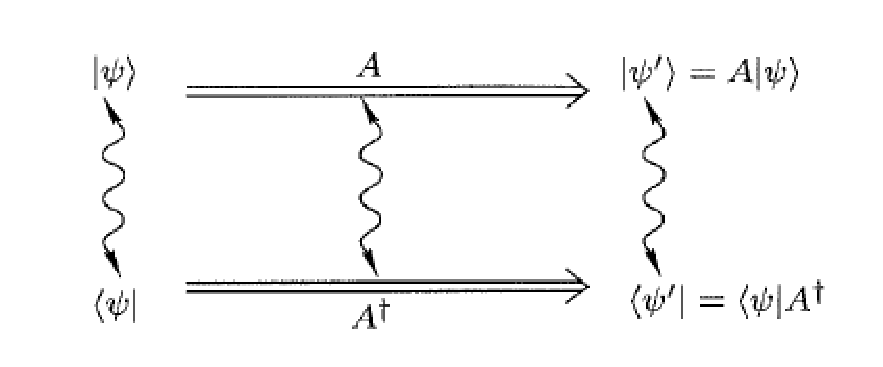
\includegraphics[scale=0.4]{fig/b-1.eps}
    \caption{从左矢右矢之间的关系出发定义伴随算符}
\end{figure}
\begin{thinknote}
    注意我们谈论算符一般都是在右矢构成的$\mathscr{E}$中讨论, 也就是说$\hat{A}^\dagger$也应该是一个$\mathscr{E}$中的算符。但是前面谈到过可以自然的将算子
    延伸定义到左作用于左矢, 按照上面图像定义, 我们确定$\hat{A}^\dagger$是通过它的左作用和$\hat{A}$本身来确定。这种定义方式物理意义更清晰, 不过直接使用数学
    上的方式定义会更加严谨, 而且也更好的去说明伴随算子的存在性和唯一性。
\end{thinknote}
\begin{proposition}{厄米共轭的运算特性}
    \begin{equation}
        \begin{gathered}
        \left(A^{\dagger}\right)^{\dagger}=A \\
        (\lambda A)^{\dagger}=\lambda^{*} A^{\dagger}( \text { $\lambda$是一个数 }) \\
        (A+B)^{\dagger}=A^{\dagger}+B^{\dagger}\\
        \boxed{(AB)^{\dagger}=B^{\dagger}A^{\dagger}}
        \end{gathered}
    \end{equation}
\end{proposition}
既然狄拉克符号的组合可以形成算子, 那么我们也可以对狄拉克符号的一个组合进行厄米共轭操作, 具体方法如下:
\begin{theorem}{狄拉克符号取共轭运算的规则}
    当一个式子中含有常数、右矢、左矢及算符时, 要得到这个式子的厄 米共轭式 (或伴随式), 必须:\\
\textbf{代换}:
$$\left\{\begin{array}{l}\text { 将常数换成其共轭复数 } \\ \text { 将右矢换成其对应的左矢 } \\ \text { 将左矢换成其对应的右矢 } \\ \text { 将算符换成其伴随算符 }\end{array}\right.$$
\textbf{反序}: 即颠倒各因子的顺序 (但常数的位置无关紧要).
\end{theorem}
所以我们说$\left|\psi\right\rangle$和$\left\langle \psi \right|$共轭, 复数的共轭正好和厄米共轭一致。在这个意义下, 厄米共轭操作就不单单对于算符了, 等式两边
只要都是狄拉克符号, 都可以直接按照上面的方法取厄米共轭, 狄拉克符号在形式运算中有很大的简便性。
\begin{thinknote}
    \textbf{例子}:  $\lambda\langle u|\hat{A}| v\rangle|w\rangle\langle\psi|$\\
    上面的符号全部取成其厄米共轭, 然后从又往左写成$|\psi\rangle\langle w|\left\langle v\left|\hat{A}^{\dagger}\right| u\right\rangle \lambda^{*}$, 注意到
    数$\left\langle v\left|\hat{A}^{\dagger}\right| u\right\rangle,\lambda^{*}$的位置是可以随便变动的, 所以最终答案为$\lambda^{*}\left\langle v\left|\hat{A}^{\dagger}\right| u\right\rangle\lambda^{*}|\psi\rangle\langle w|$
\end{thinknote}
你还可以发现左矢是反线性的, $\left\langle\lambda_1\psi_1+\lambda_2\psi_2\right| =\lambda_1^*\left\langle\psi_1\right|+\lambda_2^*\left\langle\psi_2\right|$
你只要记住对应的右矢是$\left|\lambda_1\psi_1+\lambda_2\psi_2\right\rangle$, 而这个右矢实际上是$\lambda_1\left|\psi_1\right\rangle+\lambda_2\left|\psi_2\right\rangle $, 取厄米共轭即可得到上式, 不要被这些简写了的记号弄混。

\section{态空间表象和算子的矩阵表示}
\begin{define}{表象}
    我们说在态空间中选取了一个表象就是选取了一个离散的或者连续的\textbf{正交归一基}\footnote[1]{基可以由广义右矢组成, 保证运算上的简便}, 在一组确定的基下, 我们可以使用矩阵来描述态矢量和算符。
\end{define}
我们使用狄拉克记号重新来写一下正交归一基底需要满足的正交归一和封闭性关系式

\textbf{正交归一性}:
\begin{lequation}
    \label{eq:B.12}
    \boxed{
        \begin{array}{c}
            \left \langle u_i  | u_j  \right \rangle = \delta_{ij}\\
            \left \langle w_\alpha  | w_{\alpha^\prime }  \right \rangle =\delta(\alpha -\alpha^\prime )
        \end{array}
    }
\end{lequation}

\textbf{封闭性}
\begin{lequation}
    \label{eq:B.13}
    \boxed{
        \begin{array}{c}
            P_{\{u_i\}}=\sum\limits _{i}\left | u_i  \right \rangle \left\langle u_i\right|= \mathbbm{1}\\
            P_{\{w_\alpha \}}=\int \mathrm{d}\alpha \left | w_\alpha   \right \rangle \left\langle  w_\alpha \right |=\mathbbm{1}
        \end{array}
    }
\end{lequation}

其实这个封闭性也蛮好理解, 就是这组基张成空间的投影算符刚好是恒等算符, 也就说明了$\mathscr{E}$空间和基矢量张成的空间重合, 也就说明了封闭性。

\subsection*{态矢量和算符的矩阵表示}
选取离散基表象, 右矢可以借助基向量写成:
\[\left | \psi  \right \rangle =\mathbbm{1}\left | \psi  \right \rangle =\sum\limits_{i}\left | u_i  \right \rangle \left\langle u_i|\psi  \right \rangle \]
那么我们可以将分量$v_i=\left\langle u_i|\psi  \right \rangle$排成一个列矩阵形式表示$\left|\psi\right\rangle$, 其行数为可数无穷大($\aleph_0$)
\begin{equation*}
    \begin{pmatrix}
        \left\langle u_1|\psi  \right \rangle \\
        \left\langle u_2|\psi  \right \rangle \\
        \vdots \\
        \left\langle u_i|\psi  \right \rangle\\
        \vdots 
    \end{pmatrix}
\end{equation*}

对于连续基, $\left|\psi\right\rangle=\int \mathrm{d}\alpha\left\langle w_{\alpha} \mid \psi\right\rangle$, 这个时候分量变成了一个连续函数, $c(\alpha)=\left\langle w_\alpha|\psi  \right \rangle$, 我
们还是可以将其写成一个列矩阵, 在矩阵旁边画上一个数轴, 数轴上的每一个点对应一个矩阵上的分量。
\begin{equation*}
    \alpha \longdownarrow{2.2} \left(\begin{array}{c}
    \vdots \\
    \left\langle w_{\alpha} \mid \psi\right\rangle \\
    \vdots
    \end{array}\right)
\end{equation*}

类似的, 单纯从共轭对称性来看, 我们可以把左矢按照${\left\langle u_i\right|}$展开。
\[\left\langle\varphi\right|=\left\langle\varphi\right|\mathbbm{1}=\sum\limits_{i}\left\langle\varphi| u_i\right\rangle\left\langle u_i \right| \]
这个时候我们把矩阵写成行向量, 这样定义会方便后面的矩阵运算。
\begin{equation*}
    \begin{pmatrix}
        \left \langle \varphi  | u_1 \right \rangle& \left \langle \varphi  | u_2 \right \rangle &\cdots
    \end{pmatrix} 
\end{equation*}
同理分析, 在连续基下矩阵表示为:
\begin{equation*}
    \underrightarrow{
        \begin{pmatrix}
        \cdots& \left \langle \varphi  | w_\alpha  \right \rangle &\cdots
        \end{pmatrix} 
    }
\end{equation*}
\begin{define}{矩阵元}
    我们将$\left \langle \varphi  \right |\hat A\left| \psi  \right \rangle $称为态$\left | \varphi  \right \rangle ,\left | \psi  \right \rangle $之间的矩阵元
\end{define}
一般情况下一个线性映射可以使用一个矩阵来描述, 这里对于算符, 可以用一个方阵来描述, 只不过行数和列数都是无穷大。很容易说明, 只要给定数组\[A_{ij}=\left \langle u_i  \right |\hat A\left| u_j  \right \rangle \]这也就是基之间的矩阵元, 只
是由于是算子所以定义域和值域的基相同, 由于这个数组唯一决定了基之间的对应关系, 所以也就唯一决定了一个算子。
\begin{equation*}
    \left(\begin{array}{ccccc}
        A_{11} & A_{12} & \cdots & A_{1 j} & \cdots \\
        A_{21} & A_{22} & \cdots & A_{2 j} & \cdots \\
        \vdots & \vdots & & \vdots & \\
        A_{i 1} & A_{i 2} & \cdots & A_{i j} & \cdots \\
        \vdots & \vdots & & \vdots &
        \end{array}\right)
\end{equation*}
对于连续基底, 你需要给定一个二元函数\[A\left(\alpha,\alpha^\prime\right)=\left \langle w_\alpha \right |\hat A\left| w_{\alpha^\prime}  \right \rangle \]
算符矩阵的行列使用两个正交的坐标轴去标记:
\begin{figure}[htbp]
    \centering
    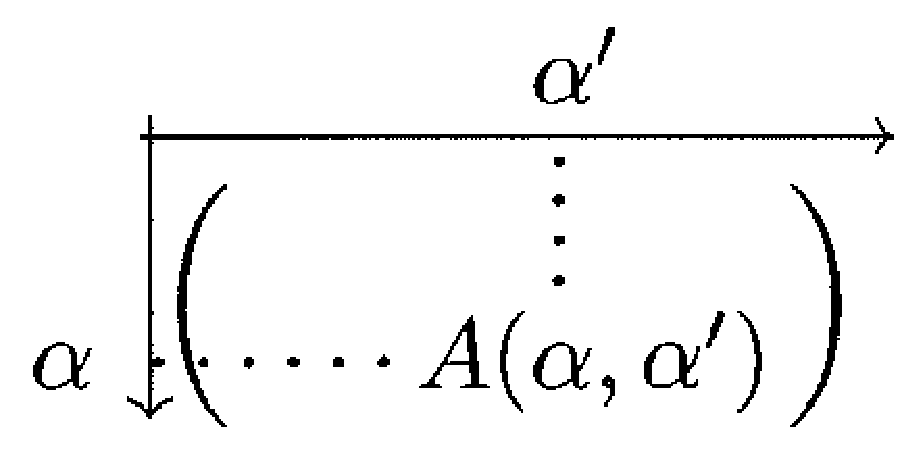
\includegraphics[width=4cm,height=2cm]{fig/b-2.eps}
\end{figure}

至此, 我们已经初步建立了算符和态矢量的矩阵表示理论, 狄拉克符号的组合也是左矢右矢或者算符, 也可以根据上面的定义去得到某基底下的矩阵表述。我们下面通过几个例子
说明, 你计算任何狄拉克符号的矩阵表述时, 只需要把所有的狄拉克符号按照顺序写下其矩阵表述, 然后\textbf{再按照矩阵的运算法则计算即可}。

\begin{equation*}
    \begin{aligned}
        \left|\psi^{\prime}\right\rangle=\hat{A}|\psi\rangle \Rightarrow c_{i}^{\prime} &=\left\langle u_{i} \mid \psi^{\prime}\right\rangle=\left\langle u_{i}|\hat{A}| \psi\right\rangle \\
        &=\left\langle u_{i}|\hat{A} \mathbbm{1}| \psi\right\rangle=\sum_{j}\left\langle u_{i}|\hat{A}| u_{j}\right\rangle\left\langle u_{j}\right| \\
        &=A_{i j} u_{j}=A_{i j} c_{j}
    \end{aligned}
\end{equation*}
\begin{thinknote}
    所以狄拉克符号中的封闭性关系真的很好用, 下面要推导的式子都不用记结论, 学会推导方法即可。
\end{thinknote}
\begin{equation*}
    \boxed{
        A^{\dagger}{ }_{i j}=\left\langle u_{i}\left|\hat{A}^{\dagger}\right| u_{j}\right\rangle=\left\langle u_{j}|\hat{A}| u_{i}\right\rangle^{*}=A_{j i}{ }^{*}
    }
    \end{equation*}
\textbf{在正交归一基下}, 对算符进行厄米共轭操作, 它的矩阵相当于转置后再取复数共轭。
\begin{define}{厄米算符/矩阵}
    若$\hat{A}^\dagger=\hat{A}$我们就趁算符$\hat{A}$是厄米的。由于我们前面说明了厄米共轭和复数共轭的相似性, 这里厄米算符也可以和实数类比。按照定义, 厄米算符的
    矩阵的对角线上元素全为实数。
\end{define}
最后推导一下投影算符的矩阵元表示:
\begin{equation*}
    P_{ij} =\left\langle u_i|\psi\right\rangle\left\langle\psi| u_j \right\rangle\rightarrow\\
    \left(\begin{array}{c}
        c_{1} \\
        c_{2} \\
        \vdots \\
        c_{i} \\
        \vdots
        \end{array}\right)\left(c_{1}^{*} c_{2}^{*} \cdots c_{j}^{*} \cdots\right)=\left(\begin{array}{ccccc}
        c_{1} c_{1}^{*} & c_{1} c_{2}^{*} & \cdots & c_{1} c_{j}^{*} & \cdots \\
        c_{2} c_{1}^{*} & c_{2} c_{2}^{*} & \cdots & c_{2} c_{j}^{*} & \cdots \\
        \vdots & \vdots & & \vdots & \\
        c_{i} c_{1}^{*} & c_{i} c_{2}^{*} & \cdots & c_{i} c_{j}^{*} & \cdots \\
        \vdots & \vdots & & \vdots &
        \end{array}\right)
\end{equation*}
这也说明了前面我们将左矢的矩阵写成行向量的好处, 计算上与矩阵完全一致了。
\subsection*{表象的变换}
选取不同的表象, 不会导致态矢量或者算符本身发生变化, 但是描述它们的矩阵会有很大的不同, 但是它们之间是有联系的, 对于算符, 这些矩阵互为相似矩阵。

令$$S_{ik}=\left\langle u_i  | t_k  \right\rangle$$称为两个基之间的变换矩阵, 下面的推导只需要使用封闭性关系就可以很容易做到。它的厄米共轭可计算为:
$$
\left(S^{\dagger}\right)_{k i}=\left(S_{i k}\right)^{*}=\left\langle t_{k} \mid u_{i}\right\rangle
$$
\begin{define}{幺正算子}
    \begin{equation}
        \boxed{U^\dagger U=U U^\dagger=I}
    \end{equation}
    则称$U$为幺正算子, 对应的矩阵称为幺正矩阵(酉矩阵)\footnote[1]{可以证明幺正算子的矩阵在任何表象下均为幺正矩阵}。它对应于实向量空间中的正交矩阵, 类比实向量空间中, 正交矩阵是一个等距同构, 正交变换恰如坐标系旋转。
\end{define}
实际上上面的变换矩阵就是一个幺正矩阵。下面利用封闭性关系插入$\mathbbm{1}$有:
\begin{equation*}
   \begin{aligned}
    A_{i j} &=\left\langle u_{i}|\mathbbm{1}A|\mathbbm{1}u_{j}\right\rangle=\left\langle u_{i}\left|P_{\left\{t_{k}\right\}} A P_{\left\{t_{l}\right\}}\right| u_{j}\right\rangle \\
    &=\sum_{k, l}\left\langle u_{i} \mid t_{k}\right\rangle\left\langle t_{k}|A| t_{l}\right\rangle\left\langle t_{l} \mid u_{j}\right\rangle \\
    &=\sum_{k, l} S_{i k} A_{k l} S_{l j}^{\dagger}
    \end{aligned} 
\end{equation*}
右矢左矢的变换也是一样的推导, 不用背公式, 使用狄拉克符号插入$\mathbbm{1}$即可。
\subsection*{线性变换矩阵的一般说明}
对于一个$V\mapsto W$的一个线性变换$T$,我们用矩阵表示它需要确定$V$和$W$中的一组基底$\{\mathbf{e}_1,\cdots\mathbf{e}_n\}$和$\{\mathbf{f}_1,\cdots\mathbf{f}_m\}$
在这样的两组基底下,线性算子$T$的矩阵记为$\mathcal{M}(T,\{\mathbf{e}_1,\cdots\mathbf{e}_n\},\{\mathbf{f}_1,\cdots\mathbf{f}_m\})$,\textbf{其第$i$列的意义是$T$作用到$e_i$上在$W$的基底$\{f\}$上的
展开系数。}

对于线性算子$T$,也就是$V\mapsto V$的线性变换,为了矩阵表示这个算子我们一般取两组相同的基底,矩阵就简记为$\mathcal{M}(T,\{\mathbf{e}_1,\cdots\mathbf{e}_n\})$,量子力学中我们最喜爱用的就是
正交归一的基底,那根据定义便有$A_{ij}=\braket{e_i|\hat{A}|e_j}$.但是别忘了这并不是一般的情况,是我们选取了正交归一的基底。而且只有在正交归一的基底选取下,才会有简单的$\hat{A}^\dagger$的矩阵等于$\hat{A}$的矩阵
的厄米共轭。

我们量子力学中考虑的表象是正交归一基底,不同的表象算符的矩阵不同,用Dirac符号可以很容易表示不同矩阵之间的关系。当然这也并不是最一般的情况,我们考虑$T:V\mapsto V$在两组不同基底下的矩阵:
\[\mathcal{M}(T,\{\mathbf{e}_1,\cdots\mathbf{e}_n\})\quad \text{and} \quad\mathcal{M}(T,\{\mathbf{f}_1,\cdots\mathbf{f}_m\})\]
恒等映射在两个基底下的矩阵记为$A=\mathcal{M}(I,\{\mathbf{e}_1,\cdots\mathbf{e}_n\},\{\mathbf{f}_1,\cdots\mathbf{f}_m\})$
\begin{theorem}{基变更公式}
    \begin{equation*}
        \mathcal{M}(T,\{\mathbf{e}_1,\cdots\mathbf{e}_n\})=A^{-1}\mathcal{M}(T,\{\mathbf{f}_1,\cdots\mathbf{f}_m\})A
    \end{equation*}
\end{theorem}
\begin{proof}
    要证明这个公式我们只需要注意到:
    \begin{align*}
        &\mathcal{M}(ST,\{u_1,\ldots,u_n\},\{w_1,\ldots,w_n\})=\\
        &\mathcal{M}(S,\{v_1,\ldots,v_n\},\{w_1,\ldots,w_n\})\mathcal{M}(T,\{u_1,\ldots,u_n\},\{v_1,\ldots,v_n\})
    \end{align*}

    这个根据定义很容易看出来,其中$S,T$都是$V$上的算子,$\{u_1,\ldots,u_n\}$和$\{w_1,\ldots,w_n\}$以及$\{v_1,\ldots,v_n\}$都是$V$的基底(不一定要正交归一).\qed
\end{proof}

我们这里所有谈到的线性代数知识更全面的了解请参看{\itshape Linear Algebra Done Right}这本书。

\section{*线性算符的一些性质}
\subsection*{本征值和本征矢}
对于$\mathscr{E}$的子空间$\mathscr{E}_q$, 如果算符$\hat{A}$将其中的矢量仍旧全部映射为$\mathscr{E}_q$中的矢量, 那么称其为算符$\hat{A}$作用下的\uwave{不变子空间}, 不
变子空间的概念在算子的分解中应用很大, 最小的不变子空间\footnote[1]{非平凡}自然是一维的, 具有下面的形式:
\[\mathscr{E}_1=\left \{ a\left|\psi\right\rangle:a\in\mathbbm{F} \right \} \]
进一步, 如果$\mathscr{E}_1$是算符$\hat{A}$的不变子空间, 则:
\begin{lequation}
    \boxed{\hat{A}\left|\psi\right\rangle=\lambda\left|\psi\right\rangle}
\end{lequation}
满足上面方程的$\lambda$称为算符的本征值, 全体本征值的集合我们称为算符$\hat{A}$的\textbf{谱}。$\left|\psi\right\rangle$称为本征矢, 本征矢不能为$\vmathbb{0}$. 每个线性无关的本征矢可以张成一个一维不变子空间。
设对于本征值$\lambda_i$有$g$个对应的线性无关的本征矢, 这些本征矢张成一个向量空间(解空间), 称为$\lambda_i$的\textbf{本征空间}, $g$正好就是本征空间的维数, 数
学上称作$\lambda_i$的几何重数\footnote[2]{还有一个对应的代数重数, 是广义本征空间的维数, 和特征多项式的解的重数相等}。在量子力学中我们称之为本征值$\lambda_i$的
\textbf{简并度}, 如果$g=1$那么我们称$\lambda_i$是\textbf{非简并}的(比如束缚态的每个能级), 反之我们称其\textbf{简并}。

选取一个表象后, 算符和矢量都可以使用矩阵来描述, 解下面的久期方程便可以很容易得到本征值和本征矢。
\begin{equation}
    \boxed{\det\left[A-\lambda I\right]=0}
\end{equation}

线性代数中对于算符的迹和行列式的定义分别为:
\[
\begin{array}{c}
    \text{tr } \hat{A} \equiv \sum \lambda \\
    \det \hat{A}\equiv \prod \lambda  
\end{array}\]

从算符在某个表象下的矩阵上定义的迹和行列式和这里的定义是相等的, 因为从矩阵出发的定义, 数学上他们被称为\uwave{相似不变量}, 物理这边可以理解为算符的矩阵的行列式和迹与你选取的表象无关。
算符的本征值肯定是不依赖于表象的, 所以数学上也给了我们在固定表象下计算迹和行列式的可行手段。

\subsection*{算符函数}
\begin{define}{以算符为自变量的函数}
    若在复数域上定义的函数可以在某个区间内展开为幂级数:
    \begin{equation}
        F(z)=\sum_{n=0}^{\infty }f_nz^n
    \end{equation}
    那么可以定义$F\left(\hat{A}\right)$为:
    \begin{equation}
        F\left(\hat{A}\right)\equiv\sum_{n=0}^{\infty }f_n\hat{A}^n
    \end{equation}
    其敛散性与$F(z)$的收敛半径和算符$\hat{A}$的本征值有关。
\end{define}

不难证明:
\begin{equation}
    \hat A\left | \psi  \right \rangle =\lambda\left | \psi  \right \rangle \Rightarrow F(\hat A)\left | \psi  \right \rangle =F(\lambda)\left | \psi  \right \rangle
\end{equation}
从上面的定义可以定义一个比较重要的算符函数, 实际上在解微分方程组中也用矩阵形式对其进行过类似的定义。
\begin{lequation}
    e^{\hat A}\equiv\sum_{n=0}^{\infty }\frac{1}{n!}\hat{A}^n=\mathbbm{1}+\hat{A}+\frac{1}{2}\hat{A}^2+\cdots
\end{lequation}
\begin{define}{BCH定理}
    若$\hat{A},\hat{B}$关于他们的对易子都是可对易的, 即:
    \[\left[\hat{A},\left[\hat{A},\hat{B}\right]\right]=\left[\hat{B},\left[\hat{A},\hat{B}\right]\right]=0\]
    则有:
    \begin{lequation}
        e^{\hat{A}}e^{\hat{B}}=e^{\hat{A}+\hat{B}+\left[\hat{A},\hat{B}\right]/2}
    \end{lequation}
    左边式子的意义根据级数的柯西乘积定义。
\end{define}

\subsection*{算符的导数}
对于$\hat{A}(t)$, 我们将其看作是一个函数, 定义域是数域, 值域是一个算符, 即$t$的映射。
\begin{define}{算符的导数}
    \begin{equation}
        \frac{ \mathrm{d}\hat{A}(t)}{\mathrm{d}t} \equiv\lim_{\Delta t \to 0} \frac{\hat{A}(t+\Delta t)-\hat{A}(t)}{\Delta t}
    \end{equation}
    “导函数”对于$t$还是一个算符
\end{define}
\begin{lequation}
    \begin{array}{l}
        \frac{\mathrm{d}}{\mathrm{dt}}(\hat{F}+\hat{G})=\frac{\mathrm{d} \hat{F}}{\mathrm{dt}}+\frac{\mathrm{d} \hat{G}}{\mathrm{dt}} \\
        \frac{\mathrm{d}}{\mathrm{dt}}(\hat{F} \hat{G})=\frac{\mathrm{d} \hat{F}}{\mathrm{dt}} \hat{G}+\hat{F} \frac{\mathrm{d} \hat{G}}{\mathrm{dt}}
    \end{array}
\end{lequation}
在某个确定的表象下\footnote[1]{基矢不随时变}, 可以证明矩阵元之间的关系为:
\begin{equation}
    \left ( \frac{\mathrm{d} \hat{A}(t) }{\mathrm{d} t}  \right )_{ij}=\frac{\mathrm{d} [\hat{A}(t)]_{ij} }{\mathrm{d} t} 
\end{equation}
也就是说, 在某个确定的表象下, \textbf{对算符求导, 就相当于把它矩阵的每个元素进行求导, 再按原位置排列}。

最后强调, 实分析中的求导公式, 在这里要小心使用, 例如, $\left[\hat{A}(t),\frac{\mathrm{d}\hat{A}}{\mathrm{d}t}\right]\neq 0$时
\[\frac{\mathrm{d} }{\mathrm{d} t}e^{\hat{A}(t) }\neq\frac{\mathrm{d} \hat{A}(t)}{\mathrm{d} x}e^{\hat{A}(t) }\]

\section{*对偶空间和对偶映射}
左矢其实是处于右矢的对偶空间之中的,现在我们用严谨的数学语言对对偶空间进行一般的简要介绍。不过我们的介绍集中于有限维向量空间,和量子力学中的Hilbert空间有所差距。

线性泛函和线性空间$V$的对偶空间$V^*$的定义与$\S$B.4中的定义是一致的,下面谈到的一堆定理如果从数学上严谨证明前摇过长,我们仅从物理上“感觉”一下。
\begin{theorem}{$\mathrm{dim} V=\mathrm{dim} V^*$}
    对于有限维向量空间$V$,其对偶空间$V^*$也是有限维的,且$\mathrm{dim} V=\mathrm{dim} V^*$. 所以他们俩也是同构的。
\end{theorem}
\begin{define}{对偶基底}
    有限维向量空间$V$的基底为$\{e_1,\ldots,e_n\}$,它们的对偶基为$V^*$中的一组基底$\{e^1,\ldots,e^n\}$,定义为:
    \begin{equation*}
        \boxed{e^i(e_j)=\delta_j^i}
    \end{equation*}
\end{define}
\begin{define}{对偶映射}
    若$T\in\mathcal{L}(V,W)$\footnote{$\mathcal{L}(V,W)$意思为所有$V\rightarrow W$的线性映射的集合},则$T$的对偶映射$T^*\in\mathcal{L}(W^*,V^*)$,满足:\footnote{$\circ$的含义为两映射的复合}
    \[\forall\varphi\in W^*,T^*(\varphi)=\varphi\circ T\]
\end{define}

不难验证对偶映射有下面的代数性质:
\begin{itemize}
    \item[$\bullet$] $\forall S,T\in\mathcal{L}(V,W)\rightarrow(S+T)^*=S^*+T^*$
    \item[$\bullet$] $\forall T\in\mathcal{L}(V,W),\lambda\in\mathbb{C}\rightarrow(\lambda T)^*=\lambda T^*$
    \item[$\bullet$] $\forall T\in\mathcal{L}(U,V),S\in\mathcal{L}(V,W)\rightarrow(ST)^*=T^*S^*$
\end{itemize}

这个对偶映射在量子力学里面是有定义的,算符$\hat{A}$从定义之初就是作用与右矢的,而作用于左矢没有定义,所以矩阵元应理解为$\braket{\varphi|\hat{A}|\psi}=\bra{\phi|(\hat{A}|\psi)}$.但是这样
未免有点麻烦,我们不妨认为定义$\hat A$作用于左矢$\bra{\phi}$的效果为:
\[\forall \ket{\psi}\in\mathscr{E},\braket{\left(\varphi|A\right)|\psi}=\braket{\varphi|\left(A|\psi\right)}\]
显然我们在悄然之间定义了一个$\hat A$的对偶映射。

\begin{theorem}{对偶映射的矩阵}
    $T\in \mathcal{L}(V,W),T^*\in\mathcal{L}(W^*,V^*)$,$V,W$基底分别为$\{e_i\},\{f_i\}$且$V^*$,$W^*$的基底取对应的对偶基底$\{e^i\},\{f^i\}$,那么按照上述基底计算的
    两映射矩阵为转置关系,即\[\mathcal{M}(T)=\left(\mathcal{M}(T^*)\right)^\mathrm{T}\]
\end{theorem}
\begin{proof}
    为了后续证明的表述简便,定义$A=\mathcal{M}(T),B=\mathcal{M}(T^*)$.

    根据线性映射矩阵的定义我们可以得到\footnote{利用爱因斯坦求和约定}:
    \[T(e_j)=A_{ij}f_i,\quad T^*(f^j)=f^j\circ T=B_{ij}e^i\]
    将$e_k$同时作用在第二个式子两端我们得到:
    \[(f^j\circ T)(e_k)=B_{ij}e^i(e_k)=B_{ij}\delta_k^i=B_{kj}\]
    而上式左端为:
    \[(f^j\circ T)(e_k)=f^j(Te_k)=f^j(A_{ik}f_i)=A_{ik}\delta^j_i=A{jk}\]
    故$A_{jk}=B_{kj}$,这正意味着$A=B^\mathrm{T}$
\end{proof}

这里并不要求基正交归一了,因为对偶空间这些概念都不必建立在内积空间之上。

\chapter{Gaussian Integral}
\section*{1-dimensional Gaussian integral}
\begin{center}
    \begin{equation*}
        \begin{aligned}
            &\int_{-\infty}^{\infty} e^{-x^{2}} d x=\sqrt{\pi}\\
            &\int_{-\infty}^{\infty} e^{-\frac{1}{2} a x^{2}+b x} d x=\sqrt{\frac{2 \pi}{a}} \exp \left(\frac{b^{2}}{2 a}\right)\\
            &\int_{-\infty}^{\infty} e^{-\frac{1}{2} a x^{2}+i b x} d x=\sqrt{\frac{2 \pi}{a}} \exp \left(-\frac{b^{2}}{2 a}\right)\\
            &I=\int_{-\infty}^{\infty} e^{-\frac{1}{2} a x^{2}+b x} d x=\sqrt{\frac{2 \pi}{a}} \exp \left(\frac{b^{2}}{2 a}\right)\\
            &\frac{\partial I}{\partial b}=\int_{-\infty}^{\infty} x e^{-\frac{1}{2} a x^{2}+b x} d x=\frac{b}{a} \sqrt{\frac{2 \pi}{a}} \exp \left(\frac{b^{2}}{2 a}\right)\\
            &\frac{\partial^{2} I}{\partial b^{2}}=\int_{-\infty}^{\infty} x^{2} e^{-\frac{1}{2} a x^{2}+b x} d x=\frac{1}{a}\left(1+\frac{b^{2}}{a}\right) \sqrt{\frac{2 \pi}{a}} \exp \left(\frac{b^{2}}{2 a}\right)\\
            &\int_{-\infty}^{\infty} x^{2} e^{-\frac{1}{2} a x^{2}} d x=\frac{1}{a} \sqrt{\frac{2 \pi}{a}}\\
            &\int_{-\infty}^{\infty} x^{4} e^{-\frac{1}{2} a x^{2}} d x=\frac{3}{a^{2}} \sqrt{\frac{2 \pi}{a}}\\
            &\int_{-\infty}^{\infty} x^{2 n} e^{-\frac{1}{2} a x^{2}} d x=\frac{(2 n-1) ! !}{a^{n}} \sqrt{\frac{2 \pi}{a}}\\
            &\int_{0}^{\infty} x^{2 n+1} e^{-a x^{2}} d x=\frac{n !}{2 a^{n+1}}\\
            &\int_{0}^{\infty} x^{n} e^{-a x^{2}} d x=\frac{\Gamma\left(\frac{n+1}{2}\right)}{2 a^{\frac{n+1}{2}}}
        \end{aligned}
    \end{equation*}
\end{center}
\section*{n-dimensional Gaussian integral (such as multivariate normal distribution)}
\begin{center}
    \begin{equation*}
        \begin{gathered}
        \int_{-\infty}^{\infty} \exp \left(-\frac{1}{2} \sum_{i, j=1}^{n} A_{i j} x_{i} x_{j}\right) d \mathbf{x}=\int_{-\infty}^{\infty} \exp \left(-\frac{1}{2} x^{T} A x\right) d \mathbf{x}=\sqrt{\frac{(2 \pi)^{n}}{\operatorname{det} A}} \\
        \int_{-\infty}^{\infty} \exp \left(-\frac{1}{2} x^{T} A x+i B^{T} x\right) d^{n} x=\sqrt{\frac{(2 \pi)^{n}}{\operatorname{det} A}} \exp \left(-\frac{1}{2} B^{T} A^{-1} B\right) \\
        \int_{-\infty}^{\infty} \exp \left(\frac{i}{2} x^{T} A x+i B^{T} x\right) d^{n} x=\sqrt{\frac{(2 \pi i)^{n}}{\operatorname{det} A}} \exp \left(-\frac{i}{2} B^{T} A^{-1} B\right) \\
        \int_{-\infty}^{\infty} \exp \left(-\frac{1}{2} \sum_{i, j=1}^{n} A_{i j} x_{i} x_{j}+\sum_{i=1}^{n} B_{i} x_{i}\right) d^{n}x\\
        =\int_{-\infty}^{\infty} \exp \left(-\frac{1}{2} x^{T} A x+B^{T} x\right) d^{n} x=\sqrt{\frac{(2 \pi)^{n}}{\operatorname{det} A}} \exp \left(\frac{1}{2} B^{T} A^{-1} B\right) \\
        \end{gathered}
    \end{equation*}
\end{center}
